\newcommand{\D}[3][]{\dfrac{\dif^{#1} #2}{\dif#3^{#1}}}
\newcommand{\Par}[3][]{\dfrac{\partial^{#1} #2}{\partial#3^{#1}}}
\tikzset{elegant/.style={smooth,thick,samples=50,cyan}}
\tikzset{eaxis/.style={->,>=stealth}}
\chapter[振动与波]{\itr{Oscillations and Waves}{振动与波}}
波是振动的传播。

在本章中,我们做以下符号上的约定:
\begin{Itemize}
    \item $\vec{F}$: Force, where $\vec{F}_{net}$ refers to the net external force.
    \item $\vec{\tau}$: Torque, where $\vec{\tau}_{net}$ refers to the net external torque.
    \item $\vec{p}$: Momentum.
    \item $\vec{L}$: Angular momentum.
    \item $U$: Potential energy.
    \item $K$: Kinetic energy.
    \item $E$: Mechanical energy.
    \item $\vec{x}$: Displacement.
\end{Itemize}
\section[平衡]{\itr{Equilibrium}{平衡}}
回忆高中物理,我们知道,振动的最基本形式——简谐振动的一大特点便是具有平衡位置。因此,在开始正式讨论振动与波之前,我们先来研究一下物体平衡的条件。

平衡的定义如下:
\begin{Itemize}
    \item \itr{Equilibrium}{平衡}: The condition of a system when neither its state of motion nor its internal energy state tends to change with time.
\end{Itemize}
通过前面章节力学部分的学习,我们知道,上面的定义可以写作以下两种形式:
$$
    \left\{\begin{aligned}
        \vec{F}_{net}=0    \\
        \vec{\tau}_{net}=0 \\
    \end{aligned}
    \right.
    \Leftrightarrow
    \left\{\begin{aligned}
        \vec{p}=Const \\
        \vec{L}=Const \\
    \end{aligned}
    \right.
    \text{,或}
    \left\{\begin{aligned}
        \frac{\mathrm{d}U}{\mathrm{d}\vec{x}}=0 \\
    \end{aligned}
    \right.
$$\par
让我们分别观察两个等价的表达式,它们分别从\textbf{受力}与\textbf{能量}的角度描述了何为“平衡”。

先从受力的角度。我们知道,物体的所受的力矩大小与转轴位置有关。那么,一个自然的问题是,平衡的物体重新选取转轴位置后,总力矩依旧为零吗?答案是肯定的。
\begin{law}[\refleaftext{prove5.1}]
    $$\left\{\begin{aligned}
            \sum\limits_{i}\vec{F}_{i}=0    \\
            \sum\limits_{i}\vec{\tau}_{i}=0 \\
        \end{aligned}
        \right.
        \Longrightarrow \sum\limits_{i}\vec{\tau}_{i,O^{\prime}}=0\text{, for any other point }O^{\prime}.
    $$
\end{law}\par
特别地,对于$\vec{p}=0,\vec{L}=0$的情况,我们称之为\itr{Static equilibrium}{静态平衡}——显然,这与坐标系的选取有关。

而从能量的角度,能量关于时间一阶导为零,根据其二阶导的符号,我们又可将其分为以下三种情况\mgnote{值得注意的是,此处的$U$是一个向量函数,因此所谓的“符号”指其 Hassian 矩阵的正定/负定/不定。}:
\begin{Itemize}
    \item \itr{Stable equilibrium}{稳定平衡}: $\D[]{U}{\vec{x}}=0,\D[2]{U}{\vec{x}}<0$
    \item \itr{Unstable equilibrium}{不稳定平衡}: $\D[]{U}{\vec{x}}=0,\D[2]{U}{\vec{x}}<0$
    \item \itr{Neutral equilibrium}{随遇平衡}: $\D[]{U}{\vec{x}}=0,\D[2]{U}{\vec{x}}=0$
\end{Itemize}

直观上讲,\itr{Stable equilibrium}{稳定平衡} 位置势能取最小值,好比是一个落入坑中的小球,在施以一定干扰的情况下是“稳定”的;\itr{Unstable equilibrium}{不稳定平衡} 位置势能取最大值,好比是一个停留在穹顶的小球,虽然静止,但一旦受到外力干扰便会打破其平衡的状态;而\itr{Neutral equilibrium}{随遇平衡}可以理解为物体的平衡状态不会被位移所改变,例如一根横躺的圆柱,无论滚到哪里都可以保持静止。
\section[振动]{\itr{Oscillations}{振动}}
\subsection[简谐运动]{\itr{Simple Harmonic Motion (SHM)}{简谐运动}}
简谐运动想必大家已经非常了解了,下面我们用另外一种方式引入。

考虑一个 \itr{Stable equilibrium}{稳定平衡} 的物体,在平衡点$\vec{x}_0$对$U$做关于$\vec{x}$的 \itr{Taylor expansion}{泰勒展开}
\[
    \begin{aligned}
        U(\vec{x}) & =U(\vec{x}_0)+\cancel{\D[]{U}{\vec{x}}\bigg|_{\vec{x}_0}(\vec{x}-\vec{x}_0)}+\frac{1}{2} \D[2]{U}{\vec{x}}\bigg|_{\vec{x}_0}(\vec{x}-\vec{x}_0)^2+\cdots \\
                   & \approx U(\vec{x}_0)+\frac{1}{2} k (\vec{x}-\vec{x}_0)^2\ ,k=\D[2]{U}{\vec{x}}\bigg|_{\vec{x}_0}\  (\vec{x} \sim \vec{x}_0)
    \end{aligned}
\]

而我们又知道$\vec{F}=-\D[]{U}{\vec{x}}$,于是得到:
\[
    \vec{F}=-k(\vec{x}-\vec{x}_0)
\]

如果将$k$近似看做一个正常数,显然,这便与我们高中接触的简谐运动的定义相同。由此可见,简谐运动实际上是一种具有更为广泛意义的运动。

下面我们给出简谐运动的完整定义:
\begin{Itemize}
    \item \itr{Simple harmonic motion}{简谐运动}: The motion of an object whose acceleration of the system, and therefore the net force, is proportional to the displacement and acts in the opposite direction of the displacement.
\end{Itemize}

利用牛顿第二定律,我们可以列出以下微分方程\mgnote{在接下来的讨论中,我们要求运动是一维的。因此,这里使用标量式}:
\[m\ddot{x}=-k(x-x_0)\]
解这个微分方程(\refleaftext{prove5.2}),得到:
\[x(t)=A\cos(\omega t+\varphi)+x_0\]
其中
\begin{Itemize}
    \item $A$: \itr{Amplitude}{振幅}, the maximum displacement from the equilibrium position.
    \item $\omega$: \itr{Angular frequency}{角频率}, which identically equals to $\sqrt{\frac{k}{m}}$.
    \item $\varphi$: \itr{Initial phase angle}{初相角}, which determines the initial position of the motion at $t=0$.
\end{Itemize}

我们再定义两个物理量:
\begin{Itemize}
    \item $T$: \itr{Period}{周期}, the time taken for one complete cycle of motion.
    \item $f$: \itr{Frequency}{频率}, the number of cycles per unit time.
\end{Itemize}
则有以下关系:
\[T=\frac{2\pi}{\omega},f=\frac{1}{T}=\frac{\omega}{2\pi}\]

而利用$x(t)=A\cos(\omega t+\varphi)+x_0$,我们可以进一步得到:
\[
    \left\{
    \begin{aligned}
        v= & -\omega A\sin(\omega t+\varphi)   & = & \ \omega A\cos(\omega t+\varphi+\frac{\pi}{2}) \\
        a= & -\omega^2 A\cos(\omega t+\varphi) & = & \ \omega^2 A\cos(\omega t+\varphi+\pi)
    \end{aligned}
    \right.
\]

两个小结论:
\begin{Itemize}
    \item 偏离平衡位置的位移与加速度符号相反。
    \item 位移、速度与加速度周期一致。
\end{Itemize}

下面,我们来讨论简谐运动物体的机械能:
\[
    \begin{aligned}
        K             & =\hspace{1.6em}\frac{1}{2}mv^2
                      &
        \hspace{-1em} & =\frac{1}{2}m\omega^2A^2\sin^2(\omega t+\varphi) \\
                      &
                      &
        \hspace{-1em} & =\frac{1}{2}kA^2\sin^2(\omega t+\varphi)         \\
        U             & =\frac{1}{2}k(x-x_0)^2
                      &
        \hspace{-1em} & =\frac{1}{2}kA^2\cos^2(\omega t+\varphi)
    \end{aligned}
\]
于是
\[E=K+U=\frac{1}{2}kA^2\]
这说明简谐运动系统总机械能守恒,且振幅大小的平方与总机械能大小正相关\footnote{不知大家此时有没有想到Parseval恒等式呢}。

对动能与势能的表达式稍加变形:
\[
    \begin{aligned}
        K & =\frac{1}{2}kA^2\frac{1-\cos(2\omega t+2\varphi)}{2} \\
        U & =\frac{1}{2}kA^2\frac{1+\cos(2\omega t+2\varphi)}{2}
    \end{aligned}
\]
即得到两者的周期均为运动周期的一半。
\subsection[用匀速圆周运动表达简谐运动]{\itr{Expressing SHM With Uniform Circular Motion}{用匀速圆周运动表达简谐运动}}
看到三角函数,我们自然会想到圆。简谐运动与匀速圆周运动之间的关系是非常直接的。
\begin{center}
    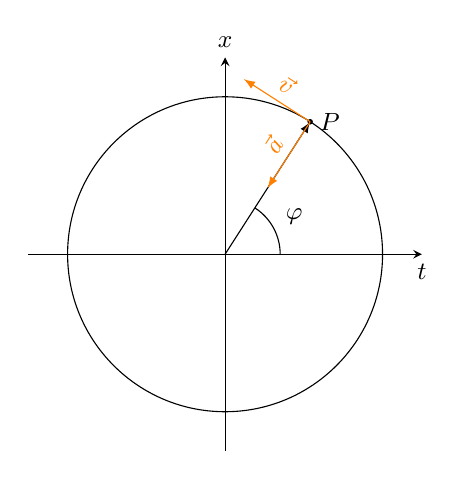
\begin{tikzpicture}
        % draw the axis
        \draw[eaxis] (-2.5,0) -- (2.5,0) node[below] {$t$};
        \draw[eaxis] (0,-2.5) -- (0,2.5) node[above] {$x$};
        % draw the function (piecewise)
        \coordinate (o) at (0,0);
        \coordinate (p) at (1.0806,1.6829);
        \coordinate (a) at (0,1);
        \coordinate (b) at (1,0);
        \draw (0,0) circle (2);
        \draw[-latex] (0,0) -- (1.0806,1.6829);
        \fill (1.0806,1.6829) circle (1pt);
        \draw (1.0806,1.6829) node[right]{$P$};
        \draw[-latex,color=orange] (1.0806,1.6829) -- node [pos=0.5,above,sloped]{$\vec{a}$} (0.5403,0.8415);
        \draw[-latex,color=orange] (1.0806,1.6829) -- node [pos=0.5,above,sloped]{$\vec{v}$} (0.2391,2.2232);
        \draw (0.7,0) arc(0:57.296:0.7);
        \draw (0.877,0.479) node{$\varphi$};
    \end{tikzpicture}\par
    \refstepcounter{figure}
    图\thefigure: 圆周运动示意图
\end{center}\par
考虑$P$点在$x$轴上的投影,显然有$x=Acos(\omega t+\varphi)$。于是我们知道,每一个简谐运动都可以与一个圆周运动相对应。这种思想将会在后续内容中有所体现。
\subsection[阻尼振动$^*$]{\itr{Damped Oscillations}{阻尼振动}$^*$}
下面我们来稍微超越一下高中范围。我们知道,生活中难以存在真正的简谐运动的一大原因是阻力的存在。我们先考虑一种最普遍的阻力——流体阻力。在低速条件下,流体阻力的大小可以由下式表达:
\[
    F_d=-bv\footnote{实际上,流体阻力公式应为$F_d=\frac{1}{2}\rho v^2C_dA$,课内要求的仅仅是解决低速情况。针对更准确的表达式,我们将在补充材料中讨论。}
\]
其中$b$被称为阻尼系数,是一个由物体形状与流体性质决定的量。直观理解,如果阻尼不大,系统的运动方式应当接近简谐运动,但是随时间会有能量的损耗;而阻尼很大时,系统可能就不能震荡了。

与解决简谐运动问题一样,我们用牛顿第二定律列出微分方程:
\begin{center}
    $m\ddot{x}=-k(x-x_0)-b\dot{x}$
\end{center}

解这个微分方程(\refleaftext{prove5.3}),会发现它的解实际上需要分为\linebreak 三类。按照物理图像的不同,我们分别称它们为:\itr{Underdamped}{欠阻尼},\itr{Overdamped}{过阻尼},\linebreak\itr{Critically damped}{临界阻尼}。

我们定义 \itr{Natural angular frequency}{固有角频率} 为 $\omega_0=\sqrt{\frac{k}{m}}$,然后有解:
\begin{Itemize}
    \item \itr{Underdamped}{欠阻尼}$(\frac{k}{m}<(\frac{b}{2m})^2)$:
    \[
        x=Ae^{-\frac{b}{2m}t}\cos(\sqrt{\frac{k}{m}-(\frac{b}{2m})^2}t+\varphi)+x_0
    \]
    \item \itr{Overdamped}{过阻尼}$(\frac{k}{m}<(\frac{b}{2m})^2)$:
    \[
        x=A_1\exp\left[\left(-\frac{b}{2m}+\sqrt{\frac{b}{2m}-(\frac{k}{m})^2}\right)t\right]+A_2\exp\left[\left(-\frac{b}{2m}-\sqrt{\frac{b}{2m}-(\frac{k}{m})^2}\right)t\right]+x_0
    \]
    \item \itr{Critically damped}{临界阻尼}$(\frac{k}{m}=(\frac{b}{2m})^2)$:
    \[
        x=(A_1+A_2t)e^{-\frac{b}{2m}}+x_0
    \]
\end{Itemize}
\begin{center}
    \begin{tikzpicture}
        % draw the axis
        \draw[eaxis] (0,0) -- (2.6*pi,0) node[below] {$t$};
        \draw[eaxis] (0,-pi/2) -- (0,pi/2) node[above] {$x$};
        % draw the function (piecewise)
        \draw[elegant,orange,domain=0:2.5*pi] plot(\x,{e^(-\x*0.3)*cos(2.5*\x r)});
        \draw[elegant,red,domain=0:2.5*pi] plot(\x,{(1-0.1*\x)*e^(-\x*0.3)});
        \draw[elegant,yellow5,domain=0:2.5*pi] plot(\x,{0.5*e^(-\x*0.1)+0.5*e^(-\x*0.3)});
    \end{tikzpicture}\par
    \refstepcounter{figure}
    图\thefigure:三种阻尼振动
\end{center}

如果阻尼较小,物体会振荡,且随着能量被阻力消耗,振幅会逐渐减小。其极限情况便是“临界阻尼”\mgnote{即恰好不发生振荡的情况} 。如果阻尼很大,质点在运动时不会振荡,而是会慢慢返回到平衡位置。

有趣的是,能量耗散最快的情况是临界阻尼。一种理解方式是考虑两种极限情况:阻尼接近零时,系统接近于简谐运动,能量几乎不消耗;阻尼无穷大时,系统接近静止,能量同样几乎不消耗。临界阻尼的这种特性被应用于电流表的阻尼设计中。

\begin{center}
    \begin{tikzpicture}
        % draw the axis
        \draw[eaxis] (0,0) -- (2.6*pi,0) node[below] {$t$};
        \draw[eaxis] (0,-pi/2) -- (0,pi/2) node[above] {$x$};
        % draw the function (piecewise)
        \draw[elegant,orange,domain=0:2.5*pi] plot(\x,{e^(-\x*0.3)*cos(2.5*\x r)});
        \draw[elegant,yellow8,domain=0:2.5*pi] plot(\x,{e^(-\x*0.3)});
        \draw[elegant,yellow8,domain=0:2.5*pi] plot(\x,{-e^(-\x*0.3)});
    \end{tikzpicture}\par
    \refstepcounter{figure}
    图\thefigure: 欠阻尼的包络线
\end{center}

对于欠阻尼的情况,还可以将其看作是能量的指数衰减与周期运动的叠加。相对于无阻尼的情况,体系的周期会增大。
\subsection[受迫振动$^*$]{\itr{Forced Oscillations}{受迫振动}$^*$}
下面让我们转向另一类常见的振动形式:
\begin{Itemize}
    \item \itr{Forced Oscillations}{受迫振动}: The condition of system when it is driven by a periodic force that is external to the oscillating system.
\end{Itemize}

在阻尼运动的基础上\mgnote{原因且埋一个伏笔},我们设驱动力的表达式为$F_d=F_{ext}\cos \omega t$。同样,我们用牛顿第二定律列出微分方程:
\[m\ddot{x}=-k(x-x_0)-b\dot{x}+F_{ext}\cos \omega t\]
解这个微分方程(\refleaftext{prove5.4}),得到:
\[x=\underbrace{A^{\prime}e^{-\frac{b}{2m}t}\cos(\omega^{\prime}t+\varphi^{\prime})}_{\text{transient solution}}+\underbrace{A\cos(\omega t-\varphi)}_{\text{steady solution}}+x_0\]
令$\omega_0=\sqrt{\frac{k}{m}}$,则其中\mgnote{$\varphi$被称为 relative phase,即相对(驱动力)的相位}
\[
    \left\{
    \begin{aligned}
        A            & =\dfrac{F_{ext}/m}{\sqrt{(\omega^2-\omega_0^2)^2+(b\omega/m)^2}} \\
        \tan \varphi & =\dfrac{b\omega/m}{\omega_0^2-\omega^2}
    \end{aligned}
    \right.
\]

观察解的表达式可以发现,当$t$很大的时候,解的前半部分因为存在指数衰减因子,几乎对$x$不起作用——于是此时物体便近似在做简谐运动,也即“稳定”了。这就是为什么解的前半部分被称为\itr{transient solution}{暂态解},后半部分被称为\itr{steady solution}{稳态解}。

下面,我们采用比较“物理”的方式来分析稳态解的一些极端表现。

将微分方程改写为
\[\ddot{x}+\dfrac{b}{m}\dot{x}+\omega^2 x+\dfrac{F_{ext}}{m}\cos \omega t=0\]
同时我们有
\[
    \left\{
    \begin{aligned}
        x        & =A\cos(\omega t-\varphi)                      \\
        \dot{x}  & =\omega A\cos(\omega t-\varphi+\frac{\pi}{2}) \\
        \ddot{x} & =\omega^2 A\cos(\omega t-\varphi+\pi)         \\
        F        & =F_{ext}\cos(\omega t)
    \end{aligned}
    \right.
\]
我们可以把以上式子中的每一项与一个简谐运动所对应,再将其分别与一个匀速圆周运动所对应。于是我们可以用这样一幅图来表达:
\begin{center}
    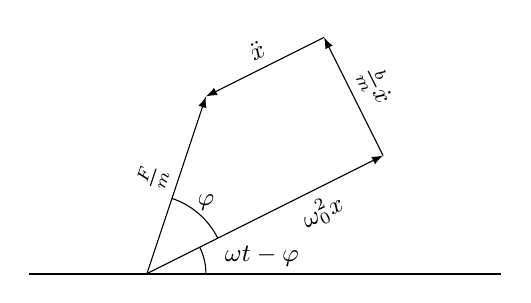
\begin{tikzpicture}[scale = 1.5]
        \draw[thick] (-1,0) -- (3,0);
        \draw[-latex] (0,0) -- node [pos=0.7,below,sloped]{$\omega_0^2 x$} (2,1);
        \draw[-latex] (2,1) -- node [pos=0.5,above,sloped]{$\frac{b}{m}\dot{x}$} (1.5,2);
        \draw[-latex] (1.5,2) -- node [pos=0.5,above,sloped]{$\ddot{x}$} (0.5,1.5);
        \draw[-latex] (0,0) -- node [pos=0.5,above,sloped]{$\frac{F}{m}$} (0.5,1.5);
        \draw (0.5,0) arc(0:26.5:0.5);
        \draw (0.9732,0.15) node{$\omega t-\varphi$};
        \draw (0.6,0.3) arc(26.5:71.5:0.6708);
        \draw (0.5,0.6) node{$\varphi$};
    \end{tikzpicture}\par
    \refstepcounter{figure}
    图\thefigure:用匀速圆周运动表达受迫振动
\end{center}\par
\refstepcounter{figure}
\begin{itemize}
    \item Slow drive $(\omega \ll \omega_0)$:\par
          此时$\dot{x},\ddot{x}$很小,于是有
          \begin{center}
              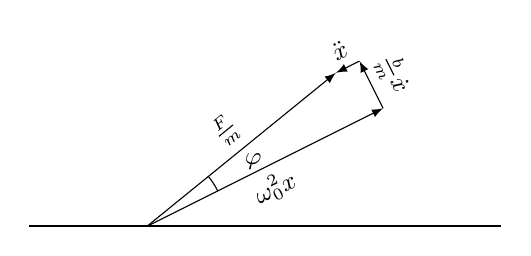
\begin{tikzpicture}[scale = 1.5]
                  \draw[thick] (-1,0) -- (3,0);
                  \draw[-latex] (0,0) -- node [pos=0.5,below,sloped]{$\omega_0^2 x$} (2,1);
                  \draw[-latex] (2,1) -- node [pos=0.5,above,sloped]{$\frac{b}{m}\dot{x}$} (1.8,1.4);
                  \draw[-latex] (1.8,1.4) -- node [pos=0.5,above,sloped]{$\ddot{x}$} (1.6,1.3);
                  \draw[-latex] (0,0) -- node [pos=0.5,above,sloped]{$\frac{F}{m}$} (1.6,1.3);
                  \draw (0.6,0.3) arc(26.5:39.1:0.6708);
                  \draw (0.9,0.55) node{$\varphi$};
              \end{tikzpicture}\par
              图\thefigure (1)
          \end{center}\par
          可以看出,$\frac{F}{m}\approx\omega_0^2 x$,也即$ F_{ext}\cos(\omega t)\approx kA\cos(\omega t-\varphi)$,这说明
          \[
              \left\{
              \begin{aligned}
                  A       & \approx \dfrac{F_{ext}}{k} \\
                  \varphi & \approx 0
              \end{aligned}
              \right.
          \]
          即物体运动与驱动力同步。
    \item Fast drive $(\omega \gg \omega_0)$:\par
          此时$\ddot{x} \gg \omega_0^2x$,于是有
          \begin{center}
              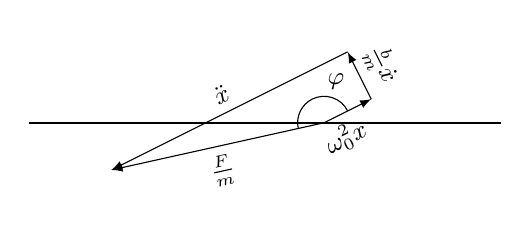
\begin{tikzpicture}[scale = 1.5]
                  \draw[thick] (-2.5,0) -- (1.5,0);
                  \draw[-latex] (0,0) -- node [pos=0.25,below,sloped]{$\omega_0^2 x$} (0.4,0.2);
                  \draw[-latex] (0.4,0.2) -- node [pos=0.5,above,sloped]{$\frac{b}{m}\dot{x}$} (0.2,0.6);
                  \draw[-latex] (0.2,0.6) -- node [pos=0.5,above,sloped]{$\ddot{x}$} (-1.8,-0.4);
                  \draw[-latex] (0,0) -- node [pos=0.5,below,sloped]{$\frac{F}{m}$} (-1.8,-0.4);
                  \draw (0.2,0.1) arc(26.5:192.5:0.2236);
                  \draw (0.1,0.35) node{$\varphi$};
              \end{tikzpicture}\par
              图\thefigure (2)
          \end{center}\par
          可以看出,$\frac{F}{m}\approx\ddot{x}$,也即$ F_{ext}\cos(\omega t)\approx mA\omega^2 \cos(\omega t-\varphi+\pi)$,这说明
          \[
              \left\{
              \begin{aligned}
                  A       & \approx \dfrac{F_{ext}/m}{\omega^2}\approx0 \\
                  \varphi & \approx \pi
              \end{aligned}
              \right.
          \]
          即物体运动与驱动力恰好反相。
    \item \itr{Resonance}{共振} $(\omega = \omega_0)$\mgnote{实际上,这是不严格的(见\refleaftext{chapter5_resonance})}:

          此时$\omega_0^2x=\ddot{x}$,于是有
          \begin{center}
              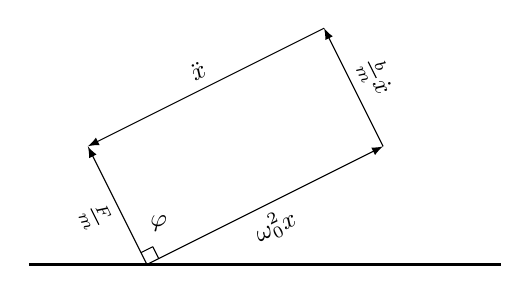
\begin{tikzpicture}[scale = 1.5]
                  \draw[thick] (-1,0) -- (3,0);
                  \draw[-latex] (0,0) -- node [pos=0.5,below,sloped]{$\omega_0^2 x$} (2,1);
                  \draw[-latex] (2,1) -- node [pos=0.5,above,sloped]{$\frac{b}{m}\dot{x}$} (1.5,2);
                  \draw[-latex] (1.5,2) -- node [pos=0.5,above,sloped]{$\ddot{x}$} (-0.5,1);
                  \draw[-latex] (0,0) -- node [pos=0.5,below,sloped]{$\frac{F}{m}$} (-0.5,1);
                  \draw (0.1,0.05) -- (0.05,0.15);
                  \draw (0.05,0.15) -- (-0.05,0.1);
                  \draw (0.1,0.35) node{$\varphi$};
              \end{tikzpicture}\par
              图\thefigure (3)
          \end{center}

          可以看出,$\frac{F}{m}=\frac{b}{m}\dot{x}$,也即$ F_{ext}\cos(\omega t)= Ab\omega \cos(\omega t-\varphi+\dfrac{\pi}{2})$,这说明
          \[
              \left\{
              \begin{aligned}
                  A       & = \dfrac{F_{ext}}{b\omega_0} \\
                  \varphi & = \dfrac{\pi}{2}
              \end{aligned}
              \right.
          \]
          此时我们便可以收回前文的伏笔:当$b\rightarrow 0$,即忽略阻尼时,与驱动力共振的物体的振幅将会达到无穷大——这显然是不可能的。
\end{itemize}
下面我们来从数学的角度对稳态解作进一步分析。
\begin{center}
    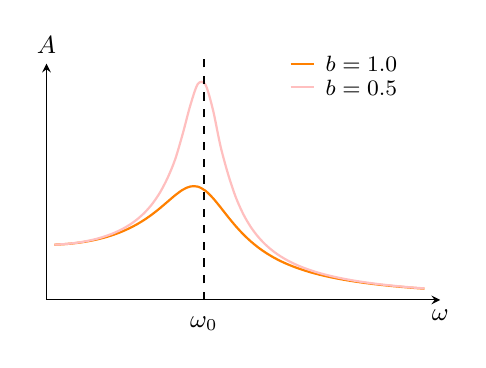
\begin{tikzpicture}
        % draw the axis
        \draw[eaxis] (0,0) -- (5,0) node[below] {$\omega$};
        \draw[eaxis] (0,0) -- (0,3) node[above] {$A$};
        % draw the function (piecewise)
        \draw[elegant,orange,domain=0.1:4.8] plot(\x,{0.7*((\x^2/4-1)^2+(\x/4)^2)^(-0.5)});
        \draw[-,thick,orange] (3.1,3) -- (3.4,3) node{};
        \node at (4, 3) {\fontsize{8}{12}$b=1.0$};
        \draw[elegant,pink,domain=0.1:4.8] plot(\x,{0.7*((\x^2/4-1)^2+(0.5*\x/4)^2)^(-0.5)});
        \node at (4, 2.7) {\fontsize{8}{12}$b=0.5$};
        \draw[-,thick,pink] (3.1,2.7) -- (3.4,2.7) node{};
        \draw[dashed] (2,0) -- (2,3.1);
        \draw (2,-0.3) node{$\omega_0$};
    \end{tikzpicture}\par
    \refstepcounter{figure}
    图\thefigure: 不同阻尼系数情况下振幅与驱动力频率的关系
\end{center}

我们很容易求出振幅$A$的极值点:
\[ \omega=\sqrt{\omega_0^2-\dfrac{b^2}{m^2}}\approx\omega_0\]

因此,物体的共振频率实际略小于物体的固有频率\labelroot{chapter5_resonance},但为了方便起见,我们一般认为它们相等。当物体处于共振状态时,振幅达到最大值;阻尼系数越接近$0$,物体的最大振幅越大:
\[ A_{max}=\dfrac{F_{ext}/b}{\sqrt{\omega_0^2-\dfrac{b^2}{m^2}}}\approx\dfrac{F_{ext}}{b\omega_0}\]
\section[波]{\itr{Waves}{波}}
\subsection[简介]{Introduction}
波随处可见。从物理的角度而言,我们将\textbf{某一物理量的扰动或振动在空间逐点传递时形成的运动}称为波。不同形式的波虽然在产生机制、传播方式和与物质的相互作用等方面存在很大差别,但在传播时却表现出多方面的共性,可用相同的数学方法描述和处理。

波可以分为以下三类:
\begin{Itemize}
    \item \itr{Mechanical Waves}{机械波}: \eg Water, Sound, \itr{Seismic Waves}{地震波}...
    \item \itr{Electromagnetic Waves}{电磁波}: \eg Light, Radio...
    \item \itr{Matter Waves}{物质波}: Quantum mechanical view of fundamental particles.
\end{Itemize}
\subsection[机械波]{\itr{Mechanical Wave}{机械波}}
下面我们主要讨论机械波。机械波的正式定义如下:
\begin{Itemize}
    \item A mechanical wave is the large movement of a disturbance in a\itr{medium}{介质}, whereas the particles that make up the medium oscillate about a fixed equilibrium position.
\end{Itemize}

机械波的形成需要以下三个条件:
\begin{enumerate}
    \item \itr{Source of disturbance}{波源}
    \item \itr{Medium}{介质}
    \item \ Physical connection between \itr{adjacent}{邻近的}\itr{portions}{部分} of the medium
\end{enumerate}
\subsection[脉冲波]{\itr{Pulse Wave}{脉冲波}}
脉冲波是一个有限长度的波。例如,如果只摇晃绳子的末端一次,则会产生脉冲波,如下图所示:
\begin{singlefigure}[Wave pulse]{chapter5_pulse_wave}[0.6]
\end{singlefigure}
我们称脉冲通过之前以及之后绳子所在的位置为 \itr{Equilibrium position}{平衡位置},称绳上质点位移的最大值为 \itr{Amplitude}{振幅}\mgnote{振幅总是非负的},用$A$表示。波的振幅由波源决定;与振动类似,波的能量与振幅正相关。

脉冲波是一种 \itr{traveling wave}{行波}。我们称 \itr{Displacement}{位移} $y$为 \itr{Wave Function}{波函数}:
\[y=f(x,t)=f(x \pm vt)\]
其中, $v$是 \itr{wave speed}{波速}, $f(x - vt)$代表 \itr{right-moving wave}{右行波}, $f(x + vt)$代表 \itr{left-moving wave}{左行波}。

出于对 \itr{polarization}{偏振} 的研究,按照振动方向与传播方向的不同关系,波又可以分为以下两类
\begin{Itemize}
    \item \itr{Transverse Wave}{横波}: A wave is transverse if the displacement from equilibrium is perpendicular to the direction the wave is traveling, or $\Delta\vec{y}\perp \vec{v}$.\par
    \quad \quad \eg Light, or the wave along a string...
    \item \itr{Longitudinal Wave}{纵波}: A material wave is longitudinal if the medium displacement from equilibrium is in the same direction that the wave is traveling, or $\Delta\vec{y}\mathrel{/\mskip-2.5mu/} \vec{v}$.\par
    \quad \quad \eg Sound, or the wave along a \itr{spring}{弹簧}...
\end{Itemize}\par
\subsection[波的叠加]{\itr{Superposition of Waves}{波的叠加}}
在满足线性近似的情况下, 波的叠加是线性的\mgnote{我们将在补充材料中证明这一点}。我们可以用下面的公式表达波的叠加:
\[y(x,t)=y_1(x,t)+y_2(x,t)\]

对于满足这一关系的波, 我们称之为 \itr{Linear Waves}{线性波};否则称之为\linebreak\itr{Nonlinear Waves}{非线性波}。线性波假设下,两束相遇的行波才可以穿过对方而不对其本身产生任何影响。

下面,我们先给出 \itr{interference}{干涉} 的定义:
\begin{Itemize}
    \item The combination of separate waves in the same region of space to produce a \itr{resultant}{合成的} wave is called interference.
\end{Itemize}

根据两束波叠加时的表现,我们将其分为以下两类:

\begin{itemize}
    \item \itr{Constructive Interference}{相长干涉}:The phenomenon where two or more waves combine to form a wave with greater amplitude.
          \begin{center}
              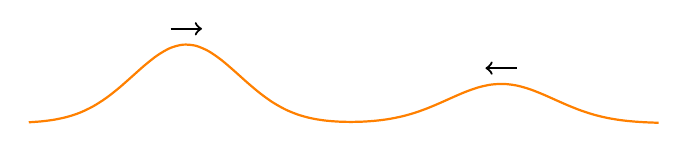
\begin{tikzpicture}
                  \draw[elegant,orange,domain=-4:4] plot(\x,{0.5*3^(-(\x-2)^2)+3^(-(\x+2)^2)});
                  \draw[->,thick] (-2.2,1.2) -- (-1.8,1.2);
                  \draw[->,thick] (2.2,0.7) -- (1.8,0.7);
              \end{tikzpicture}\par
              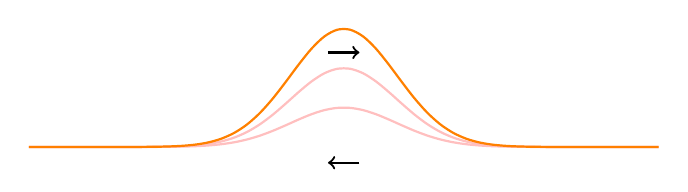
\begin{tikzpicture}
                  \draw[elegant,pink,domain=-4:4] plot(\x,{3^(-(\x)^2)});
                  \draw[elegant,pink,domain=-4:4] plot(\x,{0.5*3^(-(\x)^2)});
                  \draw[elegant,orange,domain=-4:4] plot(\x,{1.5*3^(-(\x)^2)});
                  \draw[->,thick] (-0.2,1.2) -- (0.2,1.2);
                  \draw[->,thick] (0.2,-0.2) -- (-0.2,-0.2);
              \end{tikzpicture}\par
              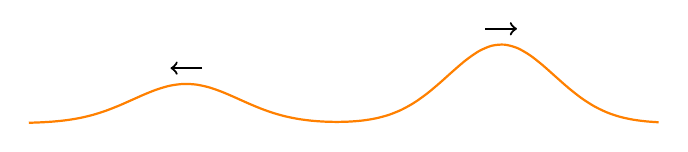
\begin{tikzpicture}
                  \draw[elegant,orange,domain=-4:4] plot(\x,{0.5*3^(-(\x+2)^2)+3^(-(\x-2)^2)});
                  \draw[->,thick] (-1.8,0.7) -- (-2.2,0.7);
                  \draw[->,thick] (1.8,1.2) -- (2.2,1.2);
              \end{tikzpicture}\par
              \refstepcounter{figure}
              图\thefigure: \itr{Constructive Interference}{相长干涉}
          \end{center}
    \item \itr{Destructive Interference}{相消干涉}:The phenomenon where two or more waves combine to form a wave with reduced or zero amplitude.
          \begin{center}
              \begin{tikzpicture}
                  \draw[elegant,orange,domain=-4:4] plot(\x,{-0.5*3^(-(\x-2)^2)+3^(-(\x+2)^2)});
                  \draw[->,thick] (-2.2,1.2) -- (-1.8,1.2);
                  \draw[->,thick] (2.2,-0.7) -- (1.8,-0.7);
              \end{tikzpicture}\par
              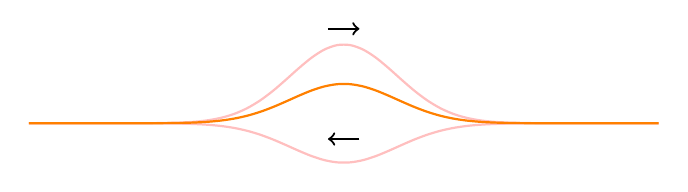
\begin{tikzpicture}
                  \draw[elegant,pink,domain=-4:4] plot(\x,{3^(-(\x)^2)});
                  \draw[elegant,pink,domain=-4:4] plot(\x,{-0.5*3^(-(\x)^2)});
                  \draw[elegant,orange,domain=-4:4] plot(\x,{0.5*3^(-(\x)^2)});
                  \draw[->,thick] (-0.2,1.2) -- (0.2,1.2);
                  \draw[->,thick] (0.2,-0.2) -- (-0.2,-0.2);
              \end{tikzpicture}\par
              \begin{tikzpicture}
                  \draw[elegant,orange,domain=-4:4] plot(\x,{-0.5*3^(-(\x+2)^2)+3^(-(\x-2)^2)});
                  \draw[->,thick] (-1.8,-0.7) -- (-2.2,-0.7);
                  \draw[->,thick] (1.8,1.2) -- (2.2,1.2);
              \end{tikzpicture}\par
              \refstepcounter{figure}
              图\thefigure: \itr{Destructive Interference}{相消干涉}
          \end{center}
\end{itemize}
\subsubsection[波的反射]{\itr{Reflection of Waves}{波的反射}}
当绳波遇到绳的端点\mgnote{介质剧烈变化的点},会发生反射现象。绳波的反射形式与端点的约束有关。一般地,我们称之为 \itr{Boundary Condition}{边界条件}。

我们先介绍最简单的两种边界条件形式:
\begin{itemize}
    \item \itr{Fixed Boundary Condition}{固定边界条件}:\par
          顾名思义,该情况对应的是绳波一个端点固定的情况。根据牛顿第三定律知,反射波将会与入射波相反。
          \begin{center}
              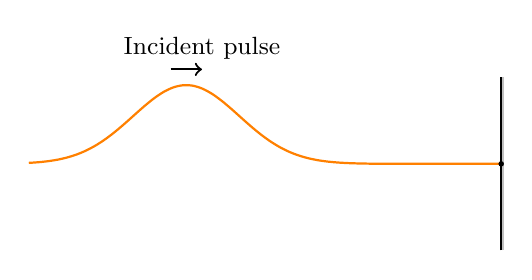
\begin{tikzpicture}
                  \draw[thick] (3,-1.1) -- (3,1.1);
                  \draw[thick, gray, opacity=0.5] (3.02,-1.1) -- (3.02,1.1);
                  \draw[elegant,orange,domain=-3:3] plot(\x,{3^(-(\x+1)^2)});
                  \draw[->,thick] (-1.2,1.2) -- (-0.8,1.2) node[above]{Incident pulse};
                  \fill (3,0) circle (1pt);
              \end{tikzpicture}\par
              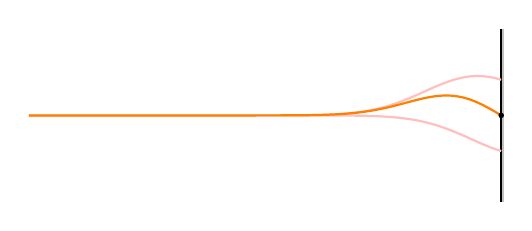
\begin{tikzpicture}
                  \draw[thick] (3,-1.1) -- (3,1.1);
                  \draw[thick, gray, opacity=0.5] (3.02,-1.1) -- (3.02,1.1);
                  \draw[elegant,pink,domain=-3:3] plot(\x,{3^(-(\x-2.7)^2)/2});
                  \draw[elegant,pink,domain=-3:3] plot(\x,{-3^(-(\x-3.3)^2)/2});
                  \draw[elegant,orange,domain=-3:3] plot(\x,{(3^(-(\x-2.7)^2)-3^(-(\x-3.3)^2))/2});
                  \fill (3,0) circle (1pt);
              \end{tikzpicture}\par
              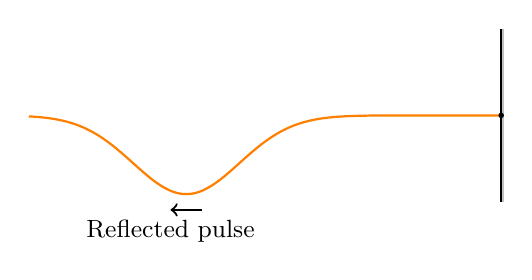
\begin{tikzpicture}
                  \draw[thick] (3,-1.1) -- (3,1.1);
                  \draw[thick, gray, opacity=0.5] (3.02,-1.1) -- (3.02,1.1);
                  \draw[elegant,orange,domain=-3:3] plot(\x,{-3^(-(\x+1)^2)});
                  \draw[->,thick]  (-0.8,-1.2)-- (-1.2,-1.2) node[below]{Reflected pulse};
                  \fill (3,0) circle (1pt);
              \end{tikzpicture}\par
              \refstepcounter{figure}
              图\thefigure: 固定边界条件下波的反射
          \end{center}
    \item \itr{Free Boundary Condition}{自由边界条件}:\par
          该情况对应的是绳波一个端点可以上下自由移动的情况(例如用一个圆环套在杆子上)。对端点进行受力分析可知,反射波将会与入射波相同。
          \begin{center}
              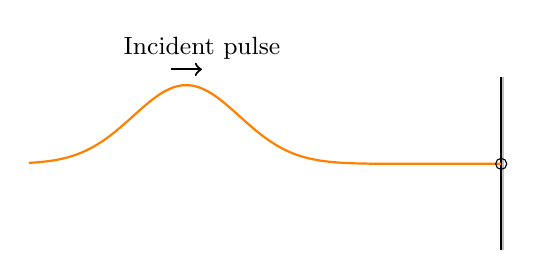
\begin{tikzpicture}
                  \draw[thick] (3,-1.1) -- (3,1.1);
                  \draw[thick, gray, opacity=0.5] (3.02,-1.1) -- (3.02,1.1);
                  \draw[elegant,orange,domain=-3:3] plot(\x,{3^(-(\x+1)^2)});
                  \draw[->,thick] (-1.2,1.2) -- (-0.8,1.2) node[above]{Incident pulse};
                  \draw (3,0) circle (2pt);
              \end{tikzpicture}\par
              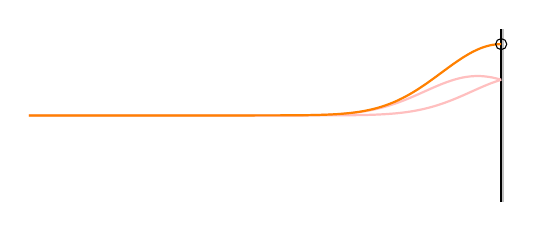
\begin{tikzpicture}
                  \draw[thick] (3,-1.1) -- (3,1.1);
                  \draw[thick, gray, opacity=0.5] (3.02,-1.1) -- (3.02,1.1);
                  \draw[elegant,pink,domain=-3:3] plot(\x,{3^(-(\x-2.7)^2)/2});
                  \draw[elegant,pink,domain=-3:3] plot(\x,{3^(-(\x-3.3)^2)/2});
                  \draw[elegant,orange,domain=-3:3] plot(\x,{(3^(-(\x-2.7)^2)+3^(-(\x-3.3)^2))/2});
                  \draw (3,0.905) circle (2pt);
              \end{tikzpicture}\par
              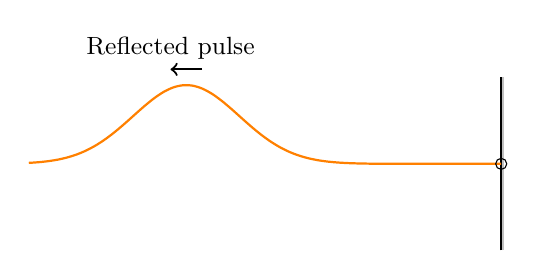
\begin{tikzpicture}
                  \draw[thick] (3,-1.1) -- (3,1.1);
                  \draw[thick, gray, opacity=0.5] (3.02,-1.1) -- (3.02,1.1);
                  \draw[elegant,orange,domain=-3:3] plot(\x,{3^(-(\x+1)^2)});
                  \draw[->,thick]  (-0.8,1.2)-- (-1.2,1.2) node[above]{Reflected pulse};
                  \draw (3,0) circle (2pt);
              \end{tikzpicture}\par
              \refstepcounter{figure}
              图\thefigure: 自由边界条件下波的反射
          \end{center}
\end{itemize}
\subsubsection[波的透射]{\itr{Transmission of Waves}{波的透射}}
我们可以将波的反射看作是极端情况下的透射(没有波成功透射)。若边界的状态介于这两种极端之间,则部分入射波会被反射,另一部分则透过边界传播。不妨记介质一中波速为$v_1$,介质二中波速为$v_2$,根据不同介质中波速的相对大小关系,我们将其分为以下两类:
\begin{itemize}
    \item $v_1>v_2$:此时波的传播接近于 \itr{Fixed Boundary Condition}{固定边界条件},发生 \linebreak\itr{Half-wave losses}{半波损失}(即反射波反相)。
          \begin{center}
              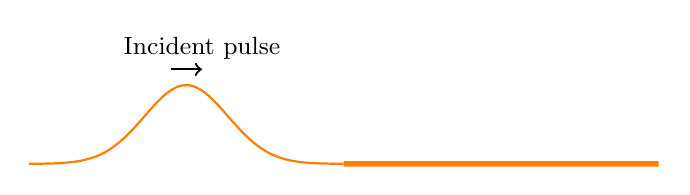
\begin{tikzpicture}
                  \draw[elegant,orange,domain=-4:0] plot(\x,{6^(-(\x+2)^2)});
                  \draw[elegant,orange,domain=0:4,line width=2pt] plot(\x,{6^(-(\x+2)^2)});
                  \draw[->,thick] (-2.2,1.2) -- (-1.8,1.2) node[above]{Incident pulse};
              \end{tikzpicture}\par
              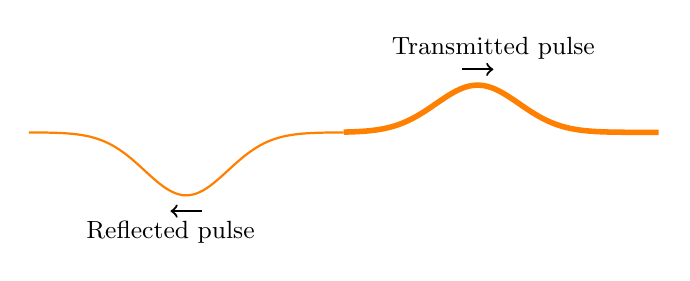
\begin{tikzpicture}
                  \tikzstyle{every node}=[font=\small]
                  \draw[elegant,orange,domain=-4:0] plot(\x,{0.8*-6^(-(\x+2)^2)});
                  \draw[elegant,thick,orange,domain=0:4,line width=2pt] plot(\x,{0.6*6^(-(\x-1.7)^2)});
                  \draw[->,thick] (-1.8,-1) -- (-2.2,-1) node[below]{Reflected pulse};
                  \draw[->,thick] (1.5,0.8) -- (1.9,0.8) node[above]{Transmitted pulse};
              \end{tikzpicture}\par
              \refstepcounter{figure}
              图\thefigure
          \end{center}
    \item $v_1<v_2$:此时波的传播接近于 \itr{Free Boundary Condition}{自由边界条件},反射波不反相。
          \begin{center}
              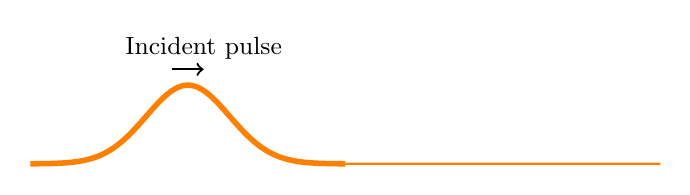
\begin{tikzpicture}
                  \draw[elegant,orange,domain=-4:0,line width=2pt] plot(\x,{6^(-(\x+2)^2)});
                  \draw[elegant,orange,domain=0:4] plot(\x,{6^(-(\x+2)^2)});
                  \draw[->,thick] (-2.2,1.2) -- (-1.8,1.2) node[above]{Incident pulse};
              \end{tikzpicture}\par
              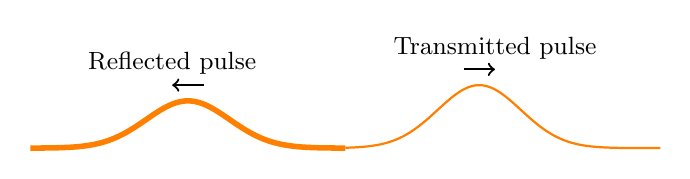
\begin{tikzpicture}
                  \draw[elegant,orange,domain=-4:0,line width=2pt] plot(\x,{0.6*6^(-(\x+2)^2)});
                  \draw[elegant,thick,orange,domain=0:4] plot(\x,{0.8*6^(-(\x-1.7)^2)});
                  \draw[->,thick] (-1.8,0.8) -- (-2.2,0.8) node[above]{Reflected pulse};
                  \draw[->,thick] (1.5,1) -- (1.9,1) node[above]{Transmitted pulse};
              \end{tikzpicture}\par
              \refstepcounter{figure}
              图\thefigure
          \end{center}
\end{itemize}
\subsection[波动方程]{\itr{Linear Wave Equation}{线性波动方程}}
在前面对脉冲波的讨论中,我们主要是从相对物理的角度来观察波传播中的现象。下面,我们通过数学的角度来严格刻画波的传播过程。

我们先介绍 \itr{phonon}{声子} 模型,描述固体材料中机械波的传播。
\begin{center}
    \begin{tikzpicture}[scale=2]
        \draw[thick] (-3,0) -- (3,0);
        \draw[dashed] (-2,1) -- (-2,-1);
        \draw[dashed] (-1,1) -- (-1,-1);
        \draw[dashed] (0,1) -- (0,-1);
        \draw[dashed] (2,1) -- (2,-1);
        \draw[dashed] (1,1) -- (1,-1);
        \fill[red] (-1.6,0) circle (2pt);
        \fill[red] (-0.7,0) circle (2pt);
        \fill[red] (-0.4,0) circle (2pt);
        \fill[red] (0.9,0) circle (2pt);
        \fill[red] (1.7,0) circle (2pt);
        \draw (-1.6,0.4) -- (-1.6,0.6);
        \draw (-2,0.4) -- (-2,0.6);
        \draw[->] (-2,0.5) -- node [pos=0.5,above,sloped]{\fontsize{8}{10}$u_{n-1}$} (-1.6,0.5);
        \draw (-0.7,0.4) -- (-0.7,0.6);
        \draw (-1,0.4) -- (-1,0.6);
        \draw[->] (-1,0.5) -- node [pos=0.5,above,sloped]{\fontsize{8}{10}$u_n$} (-0.7,0.5);
        \draw (-0.4,0.4) -- (-0.4,0.6);
        \draw (0,0.4) -- (0,0.6);
        \draw[<-] (-0.4,0.5) -- node [pos=0.5,above,sloped]{\fontsize{8}{10}$u_{n+1}$} (0,0.5);
        \draw[<->] (1,0.75) -- node [pos=0.5,above,sloped]{\fontsize{8}{10}$a$} (2,0.75);
    \end{tikzpicture}\par
    \refstepcounter{figure}
    图\thefigure:Mechanical waves in \itr{monoatomic crystal}{单原子晶体}
\end{center}

记晶格常数为$a$,则第\(n\)个声子的平衡位置$X_n=na$。再记第\(n\)个声子的实际位置为$x_n$,则它偏离平衡位置的位移为$u_n=X_n-x_n$。

为简单起见,我们只考虑相邻声子间的相互作用。记势能函数为$\psi(\Delta x)$,在$\Delta x=a$点展开,我们有
\[
    \begin{aligned}
        \psi(\Delta x) & =\psi_0+\frac{1}{2}k(\Delta x-a)^2+\cdots    \\
                       & =\psi_0+\frac{1}{2}k(x_n-x_{n-1}-a)^2+\cdots \\
                       & \approx \psi_0+\frac{1}{2}k(u_n-u_{n-1})^2
    \end{aligned}
\]
于是
\[U^{total}\approx U^{total}_0+\frac{k}{2}\sum \limits_{n}(u_n-u_{n-1})^2\]
对于第$n$个声子,我们有
\[F_n=-\D[]{U^{total}}{u_n}=k(u_{n+1}-u_n)-k(u_{n}-u_{n-1})\]
再由牛顿第二定律
\[m\ddot{u_n}=k(u_{n+1}-u_n)-k(u_{n}-u_{n-1})\]
在$\lambda \gg a$的条件下,作如下变形\mgnote{根据导数定义,容易理解这里的变形}
\[
    \begin{aligned}
        m\ddot{u_n} & =ka\frac{u_{n+1}-u_n}{a}-ka\frac{u_{n}-u_{n-1}}{a}                                                                                                           \\
                    & =ka\frac{u_{n+1}-u_n}{x_{n+1}-x_{n}}-ka\frac{u_{n}-u_{n-1}}{x_n-x_{n-1}}                                                                                     \\
                    & =ka\Par[]{u}{x}\bigg |_{x_n+\frac{a}{2}}-ka\Par[]{u}{x}\bigg |_{x_n-\frac{a}{2}}                                                                             \\
                    & =ka^2\frac{\frac{\partial u}{\partial x} \big|_{x_n+\frac{a}{2}}-\frac{\partial u}{\partial x}\big |_{x_n-\frac{a}{2}}}{(x_n+\frac{a}{2})-(x_n-\frac{a}{2})} \\
                    & =ka^2\Par[2]{u}{x}\bigg |_{x_n}                                                                                                                              \\
    \end{aligned}
\]
最后,令$v\equiv a\sqrt{\frac{k}{m}}$\mgnote{不妨思考其物理含义},我们得到了波动方程
\[\boxed{\Par[2]{u}{t}=v^2\Par[2]{u}{x}}\]

上面的推导过程是基于纵波的,下面我们基于绳波,对横波进行推导。

假设绳子的振幅很小,我们对一小段绳子进行受力分析:
\begin{center}
    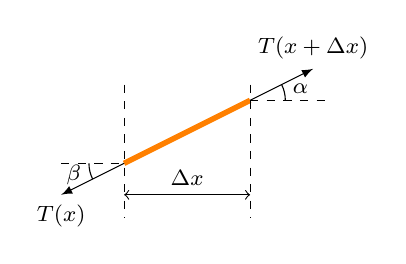
\begin{tikzpicture}[scale=2]
        \draw[line width=2pt,orange] (0,0) -- (0.8,0.4);
        \draw[dashed] (0,0.5) -- (0,-0.35);
        \draw[dashed] (0.8,0.5) -- (0.8,-0.35);
        \draw[<->] (0,-0.2) -- node [pos=0.5,above,sloped]{\fontsize{8}{10}$\Delta x$} (0.8,-0.2);
        \draw (1,0.5) arc(26.5:0:0.2236);
        \draw[dashed] (0.8,0.4) -- (1.3,0.4);
        \draw (1.12,0.475) node{\fontsize{8}{10}$\alpha$};
        \draw[-latex] (0,0) -- (-0.4,-0.2) node[below]{\fontsize{8}{10}$T(x)$};
        \draw (-0.2,-0.1) arc(180+26.5:180:0.2236);
        \draw[dashed] (-0.4,0) -- (0,0);
        \draw (-0.32,-0.075) node{\fontsize{8}{10}$\beta$};
        \draw[-latex] (0.8,0.4) -- (1.2,0.6) node[above]{\fontsize{8}{10}$T(x+\Delta x)$};
    \end{tikzpicture}\par
    \refstepcounter{figure}
    图\thefigure:对绳子的受力分析
\end{center}
$\alpha, \beta$都很小,于是有
\[
    T(x+\Delta x)\cos \alpha\approx T(x)\cos \beta \approx T
\]
记绳子的线密度为$\mu$,离开平衡位置的位移为$u$,根据牛顿第二定律,有
\[
    \begin{aligned}
        \mu\Delta x\Par[2]{u}{t} & =T(x+\Delta x)\sin \alpha-T(x)\sin \beta                  \\
                                 & \approx T\tan \alpha-T\tan \beta                          \\
                                 & =T\Par[]{u}{x}\bigg|_{x+\Delta x}-T\Par[]{u}{x}\bigg|_{x} \\
                                 & =T\Delta x \Par[2]{u}{x}
    \end{aligned}
\]
约去$\Delta x$,令$v=\sqrt{\frac{T}{\mu}}$,得到
\[\Par[2]{u}{t}=v^2\Par[2]{u}{x}\]

显然,方程的形式是完全一致的。

经过简单的验证可知,波动方程的解\mgnote{我们在 \refleaftext{prove5.5}$^*$ 给出波动方程在不同边界条件下的求解}具有以下形式
\[u=F(x+vt)+G(x-vt)\]
其中,$F(x+vt)$代表左行波,$G(x-vt)$代表右行波。

\subsection[周期波]{\itr{Periodic Wave}{周期波}}
物理世界中的波千千万,本着从简单到复杂的理念,我们先讨论一种特殊的波——周期波。而周期波中最简单的莫过于正弦波了。仿照简谐振动,我们定义以下几个物理量来描述一个正弦波。
\begin{Itemize}
    \item \itr{Amplitude}{振幅} $A$: The maximum displacement of the particle from the equilibrium position.
    \item \itr{Period}{周期} $T$: The time taken for one complete cycle of motion.
    \item \itr{Frequency}{频率} $f$: The number of cycles per unit time.
    \item \itr{Wavelength}{波长} $\lambda$: Distance of points whose oscillations differby $2\pi$.
    \item \itr{Angular frequency}{角频率} $\omega$: Which indentically equals to $\dfrac{2\pi}{T}$.
    \item \itr{Angular wave numbers}{角波数} $k$: Which indentically equals to $\dfrac{2\pi}{\lambda}$.
\end{Itemize}

根据波在一个周期内的平移,我们有关系式
\[v=\frac{\lambda}{T}=\frac{\omega}{k}\]

考虑如下正弦波:
\[
    \begin{aligned}
        y & =A\sin (kx-\omega t+\varphi)                                  \\
          & =A\sin \left[k\left(x-\frac{\omega}{k}t\right)+\varphi\right] \\
          & =A\sin \left[k\left(x-vt\right)+\varphi\right]                \\
          & =F(x-vt)
    \end{aligned}
\]
因此,$y=A\sin (kx-\omega t+\varphi)$是波动方程$\Par[2]{y}{t}=v^2\Par[2]{y}{x}$的解。

容易求得,对于该波上的一个质点,其速度\(v\)与加速度\(a\)分别为:
\[
    \begin{aligned}
        v & =\Par[]{y}{t}=-\omega A \cos(kx-\omega t+\varphi)    \\
        a & =\Par[2]{y}{t}=-\omega^2 A \sin(kx-\omega t+\varphi)
    \end{aligned}
\]
\subsubsection[能量传递速率]{\itr{Rate of Energy Transfer}{能量传递速率}}
在波动过程中,介质中的每个质点都在做简谐振动,因此波的能量包括动能和势能两部分。

设线密度为\(\mu\),我们有\(\dif m=\mu \dif x\),故质点的动能为
\[
    \dif K = \frac{1}{2} (\mu \dif x) v^2
\]
其中,$\mu \dif x$ 是质点的质量,$v$ 是质点的振动速度。

对于正弦波 $y = A \sin(kx - \omega t + \varphi)$,质点的振动速度为
\[
    v = \frac{\partial y}{\partial t} = -A \omega \cos(kx - \omega t + \varphi)
\]
因此,动能为
\[
    \dif K = \frac{1}{2} (\mu \dif x) A^2 \omega^2 \cos^2(kx - \omega t + \varphi)
\]
动能传输速率为
\[
    \D[]{K}{t} = \frac{1}{2} \mu v A^2 \omega^2 \cos^2(kx - \omega t + \varphi)
\]
从而得到动能传输速率平均值为
\[
    \left( \D[]{K}{t} \right)_{avg} = \frac{1}{4} \mu v \omega^2 A^2
\]

对于同一正弦波,势能为
\[
    \begin{aligned}
        \dif U & = T\cdot(\dif l -\dif x)
        =T\cdot\left(\sqrt{(\dif x)^2+(\dif y)^2} -\dif x\right)                      \\
               & =T\dif x\left[\sqrt{1+\left(\frac{\dif y}{\dif x}\right)^2}-1\right] \\
               & =\frac{1}{2}T\left(\frac{\dif y}{\dif x}\right)^2\dif x
        =\frac{1}{2}v^2 \mu \left(\frac{\dif y}{\dif x}\right)^2\dif x                \\
               & =\frac{1}{2}\omega^2 \mu \cos^2(kx - \omega t + \varphi)\dif x
    \end{aligned}
\]
势能传输速率为
\[
    \D[]{U}{t} = \frac{1}{2} \mu v A^2 \omega^2 \cos^2(kx - \omega t + \varphi)
\]
从而得到势能传输速率平均值为
\[
    \left( \D[]{U}{t} \right)_{avg} = \frac{1}{4} \mu v \omega^2 A^2
\]

可以发现,在波动过程中,任一质元的动能和势能相等,且同相位变化。于是质点的总能量,即其动能和势能之和,为
\[
    \dif E = \dif K + \dif U = \mu v A^2 \omega^2 \cos^2(kx - \omega t + \varphi)
\]
总能量的传输速率平均值为\labelroot{chapter5_Energy_Transfer}
\[
    \left( \D[]{E}{t} \right)_{avg} = \frac{1}{2} \mu v A^2 \omega^2
\]
\subsubsection[波的干涉]{\itr{Interference of Waves}{波的干涉}}
当两列或多列周期波在同一介质中传播时,它们会在相遇的区域产生干涉现象。此处“干涉”的要求强于我们在 \itr{Superposition of Waves}{波的叠加} 一节中讨论的。

两列周期波产生稳定干涉图样的条件是:
\begin{Itemize}
    \item 频率相同
    \item 相位差恒定
    \item 振动方向相同
\end{Itemize}
考虑两列正弦波
\[
    \begin{aligned}
        y_1 & = A \sin(kx - \omega t + \varphi_1) \\
        y_2 & = A \sin(kx - \omega t + \varphi_2)
    \end{aligned}
\]
它们的合成波为
\[
    y = y_1 + y_2 = 2A \cos\left(\frac{\varphi_2 - \varphi_1}{2}\right) \sin\left(kx - \omega t + \frac{\varphi_1 + \varphi_2}{2}\right)
\]
其中,$2A \cos\left(\frac{\varphi_2 - \varphi_1}{2}\right)$ 是合成波的振幅,取决于相位差 $\Delta \varphi = \varphi_2 - \varphi_1$。

干涉可分为以下两类:
\begin{Itemize}
    \item \itr{Constructive interference (in phase)}{相长干涉}:当两列波的相位差为 $\pi$ 的偶数倍时,振幅相加,形成加强的波。
    \item \itr{Destructive interference (out of phase)}{相消干涉}:当两列波的相位差为 $\pi$ 的奇数倍时,振幅相减,形成减弱的波。
\end{Itemize}
\subsubsection[时域相干]{\itr{Temporal Interference}{时域相干}}
下面,我们讨论更一般的情况。考虑两列正弦波:
\[
    \begin{aligned}
        y_1 & = A \sin(k_1x - \omega_1 t + \varphi_1) \\
        y_2 & = A \sin(k_2x - \omega_2 t + \varphi_2)
    \end{aligned}
\]
先假设\(v_1=v_2=v\),i.e. \(\frac{\omega_1}{k_1}=\frac{\omega_2}{k_2}=v\),有:
\[
    \begin{aligned}
        y & = y_1 + y_2                                                                                               \\
          & = A \sin(k_1x - \omega_1 t + \varphi_1) + A \sin(k_2x - \omega_2 t + \varphi_2)                           \\
          & = 2A \sin\left(\frac{(k_1x - \omega_1 t + \varphi_1) + (k_2x - \omega_2 t + \varphi_2)}{2}\right)         \\
          & \qquad \cdot \cos\left(\frac{(k_1x - \omega_1 t + \varphi_1) - (k_2x - \omega_2 t + \varphi_2)}{2}\right)
    \end{aligned}
\]
令
\[
    \omega_{avg}=\frac{\omega_1+\omega_2}{2}\quad\Delta\omega=\omega_1-\omega_2
\]
则合成波可以表示为
\[
    y = 2A \cos\left[\frac{\Delta \omega}{2}\left(\frac{x}{v}-t\right)+\frac{\varphi_1-\varphi_2}{2}\right] \sin\left[\omega_{avg}\left(\frac{x}{v}-t\right)+\frac{\varphi_1+\varphi_2}{2}\right]
\]
进一步地,我们可以这样看:
\begin{Itemize}
    \item \(\sin\left[\omega_{avg}\left(\dfrac{x}{v}-t\right)+\dfrac{\varphi_1+\varphi_2}{2}\right]\) 表示一个高频载波。
    \item \(2A\cos\left[\dfrac{\Delta \omega}{2}\left(\dfrac{x}{v}-t\right)+\dfrac{\varphi_1-\varphi_2}{2}\right]\) 表示一个低频调制波\mgnote{我们也称其为 envelop function(包络函数)}。
\end{Itemize}

如果两列波的频率接近(\(\omega_1 \approx \omega_2\)),则 \(\Delta \omega\) 很小,调制波的频率 \(\frac{\Delta \omega}{2}\) 也很小。此时,合成波会表现出明显的 \itr{beat}{拍} 现象,即振幅随时间缓慢变化,变化频率为 \(\Delta \omega\)。

\begin{center}
    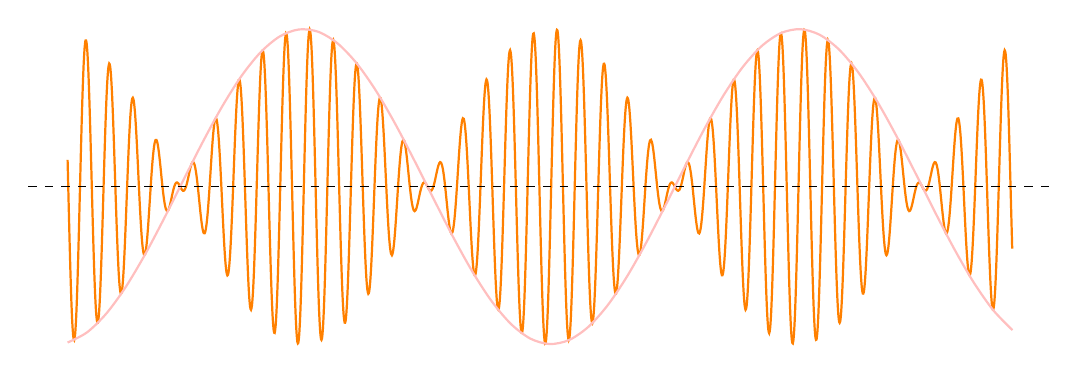
\begin{tikzpicture}
        \draw[elegant,orange,domain=-3:9,opacity=1,samples=1000] plot(\x,{sin(57.3*\x*11*2)+sin(57.3*\x*10*2)});
        \draw[elegant,pink,domain=-3:9,opacity=1] plot(\x,{2*cos(\x*0.5*57.3*2)});
        \draw[dashed] (-3.5,0) --(9.5,0);
    \end{tikzpicture}\par
    图\thefigure:合成波示意图
\end{center}

\begin{Itemize}
    \item 在小尺度上,我们有
    \[\lambda \sim \frac{2\pi}{k} \sim \frac{2\pi v}{\omega_{avg}}\]
    \item 在大尺度上,我们有
    \[\lambda' \sim \frac{2\pi v}{\Delta \omega/2}\]
\end{Itemize}

我们称
\[f_{beat}=\frac{1}{2\pi}\mid \omega_1-\omega_2\mid\]
为\itr{beat frequency}{拍频}。它可以应用于乐器调音。
\subsubsection[波包$^*$]{\itr{Wavepacket}{波包}$^*$}
进一步地,去掉\(v_1=v_2=v\)的假设,我们可以得到合成波的表达式为:
\[
    y = 2A \sin\left(\bar{k}x - \bar{\omega}t + \bar{\varphi}\right) \cos\left(\frac{\Delta k}{2}x - \frac{\Delta \omega}{2}t + \frac{\Delta \varphi}{2}\right)
\]
其中
\[
    \begin{aligned}
        \bar{k}  & = \frac{k_1 + k_2}{2}, \quad \bar{\omega} = \frac{\omega_1 + \omega_2}{2}, \quad \bar{\varphi} = \frac{\varphi_1 + \varphi_2}{2}, \\
        \Delta k & = k_1 - k_2, \quad \Delta \omega = \omega_1 - \omega_2, \quad \Delta \varphi = \varphi_1 - \varphi_2.
    \end{aligned}
\]

此时,我们得到的波函数称为一个 \itr{Wavepacket}{波包}\mgnote{针对的是其中的一个“包”}。类似于“拍”现象,Wavepacket 的运动也由小尺度上的振动与大尺度上的包络线运动所构成。我们定义下面两个物理量来描述它:
\begin{Itemize}
    \item \itr{Group Velocity}{群速度}:\(\displaystyle v_g=\frac{\Delta \omega}{\Delta k}=\frac{\dif \omega}{\dif k}\) (for \(\Delta \omega \to 0,\Delta k \to 0\))
    \item \itr{Phase Velocity}{相速度}:\( \displaystyle v_p=\frac{\omega}{k}\)
\end{Itemize}
% 上述两个速度代表 \itr{Wavepacket}{波包} 在 \itr{Phase Space}{相空间}\footnote{如有兴趣,可在补充材料里进一步讨论。}里的运动情况。
\itr{Group Velocity}{群速度} 是 Wavepacket 运动的速度,它是对 Wavepacket 运动的一阶近似。因为不同波的速度不同,Wavepacket 在运动过程中会扩散开来,于是不一定能保持其形状不变,我们便用 \itr{Dispersion relation}{色散关系}\mgnote{色散一词来自光学,不同颜色的光在同一介质中速度不同,便会发生“色散”}来描述它。通过\linebreak \itr{Phase Velocity}{相速度},我们可以对 Dispersion relation 进行分析。

根据群速度与相速度的不同,\itr{Dispersion relation}{色散关系} 分为以下三类:
\begin{Itemize}
    \item \(v_g=v_p\): \itr{Non-dispersive}{非色散} \eg Light in a vacuum.
    \item \(v_g<v_p\): \itr{Normal Dispersive}{正常色散} \eg Light in a medium.
    \item \(v_g>v_p\): \itr{Anomalous Dispersive}{反常色散}
\end{Itemize}
\begin{center}
    \begin{tikzpicture}
        \draw[elegant,orange,domain=0:2.5,opacity=1] plot(\x,{0.5*\x^2});
        \draw[->] (0,0) --  (0,4) node[left]{$k$};
        \draw[->] (0,0) --  (4,0) node[below]{$\omega$};
        \draw[dashed] (0,0) -- node[pos=0.5,above,sloped]{$v_p$} (2,2);
        \draw[dashed] (1.5,1) -- node[pos=0.5,below,sloped]{$v_g$} (2.5,3);
    \end{tikzpicture}\par
    图\thefigure: \itr{Dispersion relation}{色散关系}
\end{center}
\subsection[驻波]{\itr{Standing Wave}{驻波}}
\itr{Standing Wave}{驻波} 是两列振幅相同、频率相同、传播方向相反的波叠加形成的特殊干涉现象。

\begin{center}
    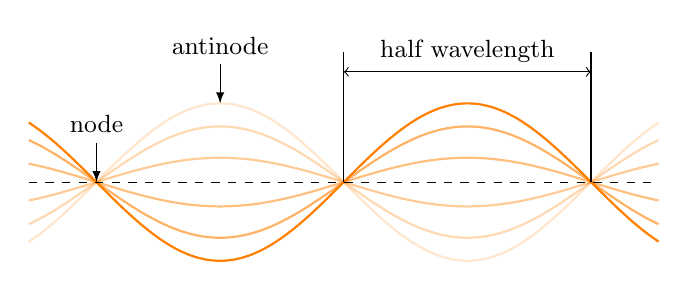
\begin{tikzpicture}
        \draw[elegant,orange,domain=-4:4,opacity=1] plot(\x,{sin(\x*57.3)*cos(0)});
        \draw[elegant,orange,domain=-4:4,opacity=0.6] plot(\x,{sin(\x*57.3)*cos(45)});
        \draw[elegant,orange,domain=-4:4,opacity=0.5] plot(\x,{sin(\x*57.3)*cos(72)});
        \draw[elegant,orange,domain=-4:4,opacity=0.4] plot(\x,{sin(\x*57.3)*cos(108)});
        \draw[elegant,orange,domain=-4:4,opacity=0.3] plot(\x,{sin(\x*57.3)*cos(135)});
        \draw[elegant,orange,domain=-4:4,opacity=0.2] plot(\x,{sin(\x*57.3)*cos(180)});
        \draw[dashed] (-4,0) --(4,0);
        \draw[-latex]  (-3.14,0.5) node[above]{\fontsize{8}{10}node} -- (-3.14,0);
        \draw[-latex]  (-3.14/2,1.5) node[above]{\fontsize{8}{10}antinode} -- (-3.14/2,1);
        \draw[<->] (0,1.4) -- node [pos=0.5,above,sloped]{\fontsize{8}{10}half wavelength} (3.14,1.4);
        \draw (0,0) -- (0,1.65);
        \draw (3.14,0) -- (3.14,1.65);
    \end{tikzpicture}\par
    图\thefigure: \itr{Standing Wave}{驻波}
\end{center}

驻波的方程为:
\[
    y = 2A \sin(kx) \cos(\omega t)
\]
驻波中,始终静止不动的点称为 \itr{Node}{波节};振幅最大的点称为 \itr{Antinode}{波腹};相邻的节点或相邻的波腹之间的距离均为 \itr{Half Wavelength}{半波长}。

驻波上每一点都在做简谐运动,没有能量传输。

驻波发生在拨动一条两端固定的弦时。
\begin{center}
    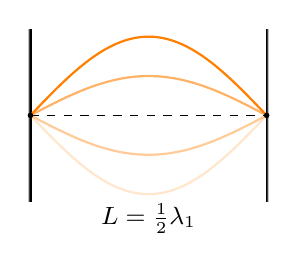
\begin{tikzpicture}
        \draw[thick] (3,-1.1) -- (3,1.1);
        \draw[thick, gray, opacity=0.5] (3.02,-1.1) -- (3.02,1.1);
        \draw[thick] (0,-1.1) -- (0,1.1);
        \draw[thick, gray, opacity=0.5] (-0.02,-1.1) -- (-0.02,1.1);
        \draw[elegant,orange,domain=0:3] plot(\x,{sin(\x*180/3)});
        \draw[dashed] (0,0) --(3,0);
        \draw[elegant,orange,domain=0:3,opacity=0.6] plot(\x,{0.5*sin(\x*180/3)});
        \draw[elegant,orange,domain=0:3,opacity=0.4] plot(\x,{-0.5*sin(\x*180/3)});
        \draw[elegant,orange,domain=0:3,opacity=0.2] plot(\x,{-sin(\x*180/3)});
        \fill (3,0) circle (1pt);
        \fill (0,0) circle (1pt);
        \draw  (1.5,-1) node[below]{$L=\frac{1}{2}\lambda_1$};
    \end{tikzpicture}
    \quad
    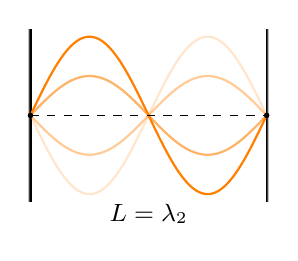
\begin{tikzpicture}
        \draw[thick] (3,-1.1) -- (3,1.1);
        \draw[thick, gray, opacity=0.5] (3.02,-1.1) -- (3.02,1.1);
        \draw[thick] (0,-1.1) -- (0,1.1);
        \draw[thick, gray, opacity=0.5] (-0.02,-1.1) -- (-0.02,1.1);
        \draw[elegant,orange,domain=0:3] plot(\x,{sin(\x*180/3*2)});
        \draw[elegant,orange,domain=0:3,opacity=0.6] plot(\x,{0.5*sin(\x*180/3*2)});
        \draw[elegant,orange,domain=0:3,opacity=0.4] plot(\x,{-0.5*sin(\x*180/3*2)});
        \draw[elegant,orange,domain=0:3,opacity=0.2] plot(\x,{-sin(\x*180/3*2)});
        \draw[dashed] (0,0) --(3,0);
        \fill (3,0) circle (1pt);
        \fill (0,0) circle (1pt);
        \draw  (1.5,-1) node[below]{$L=\lambda_2$};
    \end{tikzpicture}
    \quad
    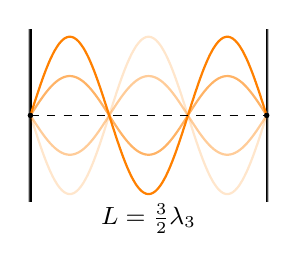
\begin{tikzpicture}
        \draw[thick] (3,-1.1) -- (3,1.1);
        \draw[thick, gray, opacity=0.5] (3.02,-1.1) -- (3.02,1.1);
        \draw[thick] (0,-1.1) -- (0,1.1);
        \draw[thick, gray, opacity=0.5] (-0.02,-1.1) -- (-0.02,1.1);
        \draw[elegant,orange,domain=0:3] plot(\x,{sin(\x*180)});
        \draw[elegant,orange,domain=0:3,opacity=0.6] plot(\x,{0.5*sin(\x*180)});
        \draw[elegant,orange,domain=0:3,opacity=0.4] plot(\x,{-0.5*sin(\x*180)});
        \draw[elegant,orange,domain=0:3,opacity=0.2] plot(\x,{-sin(\x*180)});
        \draw[dashed] (0,0) --(3,0);
        \fill (3,0) circle (1pt);
        \fill (0,0) circle (1pt);
        \draw  (1.5,-1) node[below]{$L=\frac{3}{2}\lambda_3$};
    \end{tikzpicture}\par
    \refstepcounter{figure}
    图\thefigure:两端固定情况下弦的振动
\end{center}
更一般的,我们有
\[
    \begin{aligned}
        \lambda_n & =\frac{2L}{n}       & \quad (n = 1, 2, 3, \dots) \\
        f_n       & =n\cdot\frac{v}{2L} & \quad (n = 1, 2, 3, \dots)
    \end{aligned}
\]

下面,我们考虑一个实际的场景:吉他的发声原理。

我们可以把吉他弦简单抽象为一根两个端点固定的弦
\begin{center}
    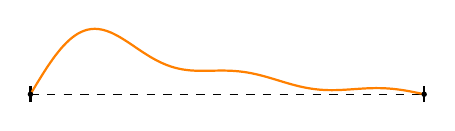
\begin{tikzpicture}
        \draw[dashed] (0,0) -- (5,0);
        \draw[thick] (0,-0.1) -- (0,0.1);
        \draw[thick] (5,-0.1) -- (5,0.1);
        \draw[elegant,orange,domain=0:5] plot(\x,{0.4*sin(\x*180/5)+0.3*sin(\x*180/5*2)+0.2*sin(\x*180/5*3)+0.14*sin(\x*180/5*4)+0.1*sin(\x*180)});
        \fill (0,0) circle (1pt);
        \fill (5,0) circle (1pt);
    \end{tikzpicture}\par
    \refstepcounter{figure}
    图\thefigure: 吉他弦的振动
\end{center}\par

吉他弦的振动产生了声音。声音的三个基本要素是 \itr{Pitch}{音高}、\itr{Loudness}{响度} 和 \itr{Timbre}{音色}。音高由频率决定,频率越高,音高越高;响度由振幅决定,振幅越大,声音越响;音色则由波形决定,不同的波形会产生不同的音色。

吉他弦的振动不仅包含基频$f_1$,还包含一系列整数倍\footnote{这是因为两端点固定情况下只允许驻波解。下学期的量子力学将会从这个角度得到量子化。}于基频的\linebreak \itr{Harmonics}{泛音}。这些泛音构成了 \itr{Harmonic Series}{泛音列},其频率为:
\[
    f_n = n \cdot f_1 \quad (n = 1, 2, 3, \dots)
\]
其中,$f_1$是基频,$f_2, f_3, \dots$分别是第二、第三泛音,依此类推。

为了更直观地理解泛音列,我们可以将声音的频域表示画出来。下图展示了图\thefigure 所示吉他弦的频域分布:

\begin{center}
    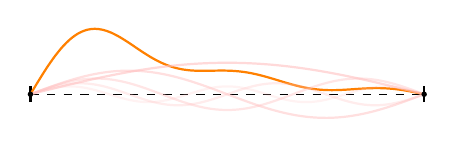
\begin{tikzpicture}
        \draw[dashed] (0,0) -- (5,0);
        \draw[thick] (0,-0.1) -- (0,0.1);
        \draw[thick] (5,-0.1) -- (5,0.1);
        \draw[elegant,orange,domain=0:5] plot(\x,{0.4*sin(\x*180/5)+0.3*sin(\x*180/5*2)+0.2*sin(\x*180/5*3)+0.14*sin(\x*180/5*4)+0.1*sin(\x*180)});
        \draw[elegant,pink,domain=0:5,opacity=0.6] plot(\x,{0.4*sin(\x*180/5)});
        \draw[elegant,pink,domain=0:5,opacity=0.5] plot(\x,{0.3*sin(\x*180/5*2)});
        \draw[elegant,pink,domain=0:5,opacity=0.4] plot(\x,{0.2*sin(\x*180/5*3)});
        \draw[elegant,pink,domain=0:5,opacity=0.3] plot(\x,{0.14*sin(\x*180/5*4)});
        \draw[elegant,pink,domain=0:5,opacity=0.2] plot(\x,{0.1*sin(\x*180)});
        \fill (0,0) circle (1pt);
        \fill (5,0) circle (1pt);
    \end{tikzpicture}\par
    \refstepcounter{figure}
    图\thefigure: 吉他弦的振动
\end{center}

\begin{center}
    \begin{tikzpicture}
        \draw[->] (0,0) -- (6,0) node[below]{$f$};
        \draw[->] (0,0) -- (0,3) node[left]{$A$};
        \foreach \x in {1,2,3,4,5} {
                \draw (\x,0) -- (\x,0.1) node[below]{$f_\x$};
            }
        \draw[thick, orange] (1,0) -- (1,2) node[above]{$A_1$};
        \draw[thick, orange] (2,0) -- (2,1.5) node[above]{$A_2$};
        \draw[thick, orange] (3,0) -- (3,1) node[above]{$A_3$};
        \draw[thick, orange] (4,0) -- (4,0.7) node[above]{$A_4$};
        \draw[thick, orange] (5,0) -- (5,0.5) node[above]{$A_5$};
    \end{tikzpicture}
    \refstepcounter{figure}\par
    图\thefigure: 吉他弦振动的频域表示
\end{center}

从图中可以看出,泛音的振幅随着频率的增加逐渐减小。通过调整弦的材料、张力以及演奏方式,可以改变泛音的分布,从而产生不同的音色效果——这也就是不同乐器音色不同的真正原因。如何求得频域表示?我们通过傅里叶变换来实现。

\subsubsection[傅里叶分析$^*$]{\itr{Fourier Analysis}{傅里叶分析}$^*$}

任何周期性振动都可以通过 \itr{Fourier Series}{傅里叶级数} 展开为一系列正弦波的叠加:
\[
    \begin{aligned}
        f(t) & = \sum_{n=0}^{+\infty} \left[A_n \cos \left(n\frac{2\pi}{T} t\right)+B_n \sin \left(n\frac{2\pi}{T} t\right)\right] \\
             & = A_0 + \sum_{n=1}^{+\infty} \left[A_n \cos (n\omega t)+B_n \sin (n\omega t)\right]
    \end{aligned}
\]
其中\mgnote{证明见 \refleaftext{prove5.6}}
\[
    \begin{aligned}
        A_0 & =\frac{1}{T}\int^T_0f(t)\dif t                                            \\
        A_n & =\frac{2}{T}\int^T_0f(t)\cos (n\omega t)\dif t \quad (n = 1, 2, 3, \dots) \\
        B_n & =\frac{2}{T}\int^T_0f(t)\sin (n\omega t)\dif t \quad (n = 1, 2, 3, \dots)
    \end{aligned}
\]

根据欧拉公式,我们也可以把傅里叶级数写成如下形式:
\[
    f(t)=\sum_{n=-\infty}^{+\infty} Z_ne^{in\omega t},\quad Z_n=\frac{1}{T}\int^T_0 f(t)e^{-in\omega t}\dif t
\]

对于非周期函数(如脉冲波),我们可以把它看做是周期为无穷大的函数。通常意义下的傅里叶级数没有意义,但是经过一些推导\mgnote{见 \refleaftext{prove5.7}},我们可以得到称为 \itr{Fourier transform}{傅里叶变换} 的结果
\[
    \begin{aligned}
        F(\omega) & =\int^{+\infty}_{-\infty}f(t)e^{-i\omega t}\dif t                        \\
        f(t)      & =\frac{1}{2\pi}\int^{+\infty}_{-\infty}F(\omega)e^{i\omega t}\dif \omega
    \end{aligned}
\]
它们也被记作\[
    \begin{aligned}
        F(\omega) & =\mathcal{F}[f(t)]           & \text{傅里叶变换}  \\
        f(t)      & =\mathcal{F}^{-1}[F(\omega)] & \text{傅里叶逆变换}
    \end{aligned}
\]

傅里叶变换实际沟通了时域与频域,具有十分重要的意义。限于篇幅,仅做简介。


\subsection[弹性]{\itr{Elasticity}{弹性}}
弹性是介质在外力作用下发生形变,并在外力撤去后恢复原状的性质。了解介质的弹性性质,有利于我们之后理解声波。

我们先介绍两个概念:

\begin{Itemize}
    \item \itr{Stress}{应力}:Deferming force per area.
    \item \itr{Strain}{应变}:Unit \itr{deformation}{形变}.
\end{Itemize}

对于小应力,我们有:
\[
    \text{Stress}=\text{Modulus(模量)}\times\text{Strain}
\]

根据外力作用方式的不同,弹性可以分为以下几类:
\begin{Itemize}
    \item \itr{Tension}{拉伸} \& \itr{Compression}{压缩}:
    当介质受到拉伸或压缩时,其长度发生变化。
    \begin{itemize}
        \item \itr{Stress}{应力}:\(F/A\)
        \item \itr{Strain}{应变}:\(\Delta L / L\)
    \end{itemize}
    其中,\(F\) 是作用力,\(A\) 是横截面积,\(\Delta L\) 是长度变化,\(L\) 是原长。
    对应的模量为 \itr{Young's Modulus}{杨氏模量} \(E\):
    \[
        E = \frac{F/A}{\Delta L / L}
    \]
    \item \itr{Shearing}{剪切}:
    当介质受到切向力作用时,其形状发生变化。
    \begin{itemize}
        \item \itr{Stress}{应力}:\(F/A\)
        \item \itr{Strain}{应变}:\(\Delta x / L\).
    \end{itemize}
    对应的模量为\itr{Shear Modulus}{剪切模量} \(G\),定义为:
    \[
        G = \frac{F/A}{\Delta x / L}
    \]
    其中,\(\Delta x\) 是切向位移,\(L\) 是介质高度。
    \item \itr{Hydraulic Stress}{液压应力}:
    当介质受到均匀压力时,其体积发生变化。
    \begin{itemize}
        \item \itr{Hydraulic Stress}{应力}:\(\Delta P\)
        \item \itr{Strain}{应变}:\(\Delta V / V\).
    \end{itemize}
    对应的模量为 \itr{Bulk Modulus}{体积模量} \(B\),定义为:
    \[
        B = -\frac{\Delta P}{\Delta V / V}
    \]
    其中,\(\Delta P\) 是压力变化,\(\Delta V\) 是体积变化,\(V\) 是原体积。
\end{Itemize}

\subsubsection[应力-应变曲线]{\itr{Stress-Strain Curve}{应力-应变曲线}}
应力-应变曲线描述了介质在外力作用下的形变行为。典型曲线包括弹性区域、屈服点、塑性区域和断裂点。

\begin{center}
    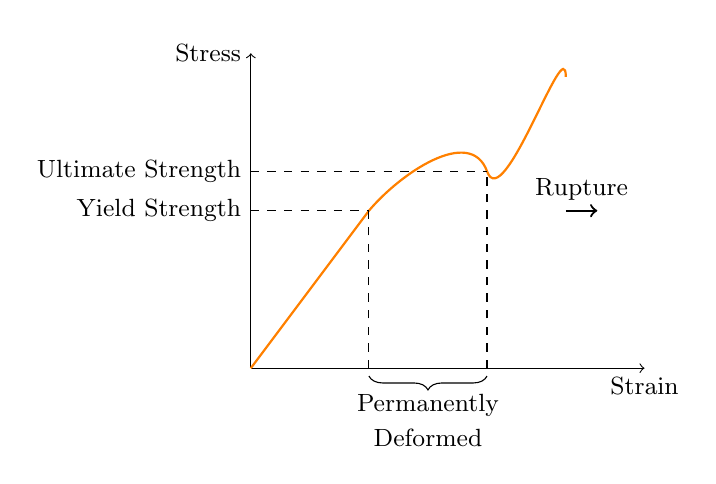
\begin{tikzpicture}
        \draw[->] (0,0) -- (5,0) node[below]{Strain};
        \draw[->] (0,0) -- (0,4) node[left]{Stress};

        \draw[thick, orange] (0,0) -- (1.5,2) to[out=50,in=110] (3,2.5) to[out=-70,in=90] (4,3.7);
        \draw[dashed] (0,2) node[left]{Yield Strength} -- (1.5,2);
        \draw[dashed] (0,2.5) node[left]{Ultimate Strength} -- (3,2.5);
        \draw[dashed] (1.5,0) -- (1.5,2);
        \draw[dashed] (3,0) -- (3,2.5);
        \draw[decorate,decoration={brace,mirror,amplitude=5pt}] (1.5,-0.1) -- (3,-0.1);
        \draw  (2.25,-0.2) node[below]{Permanently};
        \draw  (2.25,-0.65) node[below]{Deformed};
        \draw[->,thick] (4,2) -- (4.4,2) node[midway,above]{Rupture};
    \end{tikzpicture}\par
    \refstepcounter{figure}
    图\thefigure: 应力-应变曲线
\end{center}
\subsection[声波]{\itr{Sound Wave}{声波}}

声波是一种机械波,通过介质中的弹性振动传播。

\subsubsection[声波的定义]{\itr{The Definition of Sound Wave}{声波的定义}}

一切(机械)纵波都可以称为声波。声波的传播需要介质,不能在真空中传播。描述声波,我们可以使用 \itr{Wavefront}{波前} 这一概念。

\itr{Wavefront}{波前} 是声波传播过程中\textbf{相位相同}的点构成的曲面。波前的形状取决于声源的几何形状和传播介质的性质。

\begin{center}
    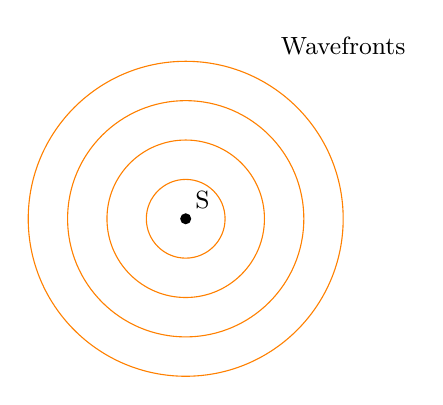
\begin{tikzpicture}
        % 点声源波前
        \fill (0,0) circle (2pt) node[above right]{S};
        \foreach \r in {0.5,1,1.5,2} {
                \draw[orange] (0,0) circle (\r);
            }
        \node at (2,2.2) {Wavefronts};
    \end{tikzpicture}\par
    \refstepcounter{figure}
    图\thefigure: 波前示意图
\end{center}

\subsubsection[声速]{\itr{Speed of Sound}{声速}}
空气中的声速 \(v\) 可以通过介质的弹性性质和密度推导得出。
\begin{center}
    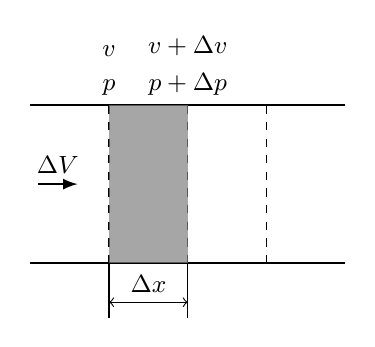
\begin{tikzpicture}
        \draw[thick] (-2,0) -- (2,0) ;
        \draw[thick] (-2,2) -- (2,2) ;
        \draw[dashed] (-1,2) node[above]{$p$} -- (-1,0) ;
        \draw (-1,2.5) node[above]{$v$};
        \draw[dashed] (0,2) node[above]{$p+\Delta p$} -- (0,0) ;
        \draw (0,2.5) node[above]{$v+\Delta v$};
        \draw[dashed] (1,2) -- (1,0) ;
        \draw[-latex,thick] (-1.9,1)--(-1.4,1) node[midway,above]{$\Delta V$};
        \fill[color=gray,opacity=0.7](-1,0)rectangle(0,2);
        \draw (0,0)--(0,-0.7);
        \draw (-1,0)--(-1,-0.7);
        \draw[<->] (-1,-0.5)--(0,-0.5) node[midway,above]{$\Delta x$};
    \end{tikzpicture}\par
    \refstepcounter{figure}
    图\thefigure: 空气压缩示意图
\end{center}

设空气从左往右运动,截面积为\(A\),密度为\(\rho\),体积模量为\(B\)。

左侧空气对右侧空气进行压缩,使得接触面速度减小(\(\Delta v<0\)),压强增大(\(\Delta p>0\))。根据牛顿第二定律,我们有:
\[
    \begin{aligned}
        F                            & =ma                                        \\
        \Rightarrow[p-(p+\Delta p)]A & =(\rho\Delta x A)\frac{\Delta v}{\Delta t} \\
        \Rightarrow -\Delta pA       & =\rho A v\Delta v
    \end{aligned}
\]
易知空气体积为\(V=A\Delta x=A v\Delta t\),体积变化量为\(V=A\Delta v\Delta t\),于是有
\[
    \frac{\Delta V}{V}=\frac{A v\Delta t}{A\Delta v\Delta t}=\frac{\Delta v}{v}
\]
进一步,我们有
\[
    \begin{aligned}
        \Delta p            & =\rho v\Delta v                 \\
        \Rightarrow\Delta p & =\rho v^2\frac{\Delta V}{V}     \\
        \Rightarrow\rho v^2 & =-\frac{\Delta p}{\Delta V/V}=B
    \end{aligned}
\]
最终得到
\[
    v=\sqrt{\frac{B}{\rho}}
\]
\subsubsection[声强]{\itr{Intensity}{声强}}
声强 \(I\) 是单位时间内通过单位面积的声能,定义为:
\[
    I = \frac{P}{A}
\]
其中,\(P\) 是声功率,\(A\) 是面积。

对于正弦波,我们有
\[
    S=A\sin(kx-\omega t+\varphi)
\]

根据 \refleaftext{chapter5_Energy_Transfer} 的结果,我们有
\[
    I=\frac{1}{2}\rho v\omega^2 A^2
\]

根据能量守恒,对于点声源,我们有
\[
    I=\frac{P_s}{4\pi r^2}
\]
其中,\(P_s\)是声源功率,\(r\)是到声源的距离。

声强与声压$^*$\mgnote{介质中有声场时的压强\(p_1\)与没有声场时的压强\(p_0\)之差为声压 \(p\)}的关系为:
\[
    I = \frac{p^2}{2\rho v}
\]

\subsubsection[声级]{\itr{Sound Level}{声级}}
声级 \(L\) 是声强的对数尺度表示,单位为分贝(dB),定义为:
\[
    L = 10 \log_{10}\left(\frac{I}{I_0}\right)
\]
其中,\(I_0 = 10^{-12} \text{W/m}^2\) 是参考声强。

\subsection[多普勒效应]{\itr{Doppler Effect}{多普勒效应}}
多普勒效应描述了声源和观察者相对运动时频率的变化。设观察者速度为\(v_D\),声源速度为\(v_S\),声速为\(v\),分以下情况讨论:
\begin{itemize}
    \item Both Stationary:
          \begin{center}
              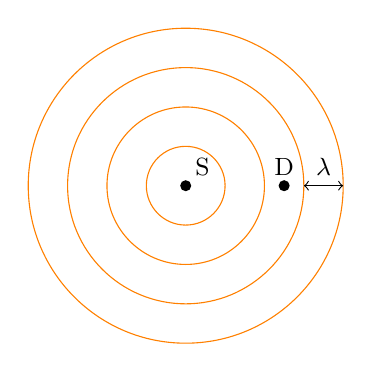
\begin{tikzpicture}
                  \fill (0,0) circle (2pt) node[above right]{S};
                  \fill (1.25,0) circle (2pt) node[above]{D};
                  \foreach \r in {0.5,1,1.5,2} {
                          \draw[orange] (0,0) circle (\r);
                      }
                  \draw[<->] (1.5,0) -- (2,0) node[midway,above]{$\lambda$};
              \end{tikzpicture}\par
              \refstepcounter{figure}
              图\thefigure: (1)
          \end{center}

          频率\(f\)是单位时间通过观察者的波前数量。显然,此时我们有
          \[
              f=\frac{vt/\lambda}{t}=\frac{v}{\lambda}
          \]

    \item Source stationary, Detector moving:
          \begin{center}
              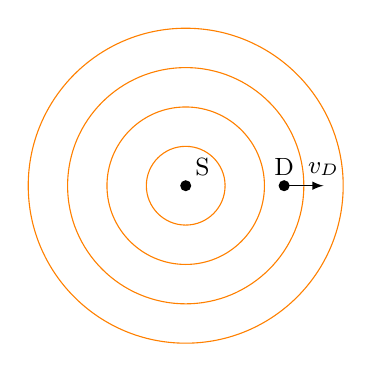
\begin{tikzpicture}
                  \fill (0,0) circle (2pt) node[above right]{S};
                  \fill (1.25,0) circle (2pt) node[above]{D};
                  \foreach \r in {0.5,1,1.5,2} {
                          \draw[orange] (0,0) circle (\r);
                      }
                  \draw[-latex] (1.25,0) -- (1.75,0) node[above]{$v_D$};
              \end{tikzpicture}\par
              图\thefigure: (2)
          \end{center}

          此时我们有
          \[
              f'=\frac{(v\pm v_D)t/\lambda}{t}=\frac{v\pm v_D}{\lambda}=\frac{v\pm v_D}{v}f
          \]

    \item Detector stationary, Source moving:
          \begin{center}
              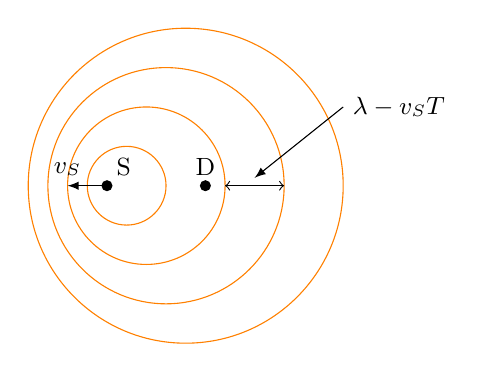
\begin{tikzpicture}
                  \fill (0,0) circle (2pt) node[above right]{S};
                  \fill (1.25,0) circle (2pt) node[above]{D};
                  \foreach \r in {0.5,1,1.5,2} {
                          \draw[orange] (\r*0.5,0) circle (\r);
                      }
                  \draw[-latex] (0,0) -- (-0.5,0) node[above]{$v_S$};
                  \draw[<->] (1.5,0) -- (2.25,0) ;
                  \draw[-latex] (3,1) node[right]{$\lambda-v_ST$} -- (1.875,0.1);
              \end{tikzpicture}\par
              图\thefigure: (2)
          \end{center}

          此时我们有
          \[
              f'=\frac{vt/(\lambda\pm v_ST)}{t}=\frac{v}{vT\pm v_ST}=\frac{v}{v\pm v_S}f
          \]

    \item Both moving:

          综合以上情况,得
          \[
              f'=\frac{v\pm v_D}{v\pm v_S}f
          \]
\end{itemize}

在 \itr{supersonic speeds}{超音速} 的情况下,波前会出现一些有趣的现象:
\begin{itemize}
    \item \(v_S=v\):
          \begin{center}
              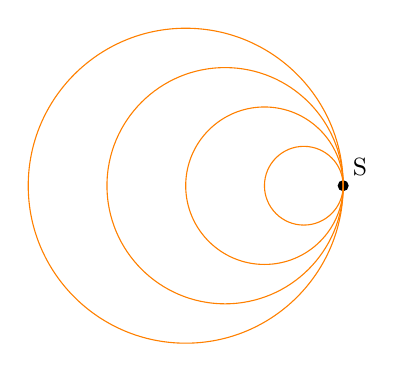
\begin{tikzpicture}
                  \fill (0,0) circle (2pt) node[above right]{S};
                  \foreach \r in {0.5,1,1.5,2} {
                          \draw[orange] (-\r,0) circle (\r);
                      }
              \end{tikzpicture}\par
              \refstepcounter{figure}
              图\thefigure: (1)
          \end{center}
          可见,波前都在声源处堆积,出现 \itr{sound barrier}{音障现象}。
    \item \(v_S>v\) (\itr{Shock Wave}{激波}):
          \begin{center}
              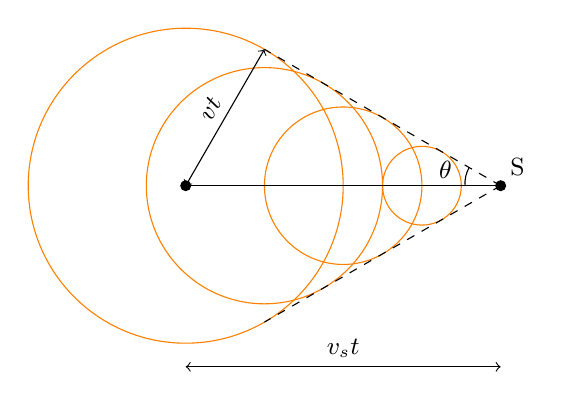
\begin{tikzpicture}
                  \fill (0,0) circle (2pt) node[above right]{S};
                  \fill (-4,0) circle (2pt) ;
                  \foreach \r in {0.5,1,1.5,2} {
                          \draw[orange] (-\r*2,0) circle (\r);
                      }
                  \draw (-4,0)--(0,0);
                  \draw[dashed] (0,0)--(-3,1.732);
                  \draw[dashed] (0,0)--(-3,-1.732);
                  \draw[<->] (-4,0)--node [pos=0.5,above,sloped]{$vt$} (-3,1.732);
                  \draw[<->] (-4,-2.3)--node [pos=0.5,above,sloped]{$v_st$} (0,-2.3);
                  \draw (-0.4,0.4/1.732) arc(150:185:0.4);
                  \draw (-0.7,0.2) node{$\theta$};
              \end{tikzpicture}\par
              \refstepcounter{figure}
              图\thefigure: (2)
          \end{center}
          我们称波前的包络面为\itr{Mach Cone}{马赫锥},并且有
          \begin{itemize}
              \item \itr{Mach Cone Angle}{马赫锥角}:\(\displaystyle \theta=\arcsin \frac{vt}{v_St}=\arcsin \frac{v}{v_S}\)
              \item \itr{Mach Number}{马赫数}:\(\displaystyle  \frac{v_S}{v}\)
          \end{itemize}
\end{itemize}
%\end{document}